\documentclass[14pt, a4paper]{article}
\usepackage{minitoc}
\usepackage[left=3.00cm, right=2.5cm, top=2.00cm, bottom=2.00cm]{geometry}
\usepackage{amsmath}
\usepackage{amssymb}
\usepackage{amsthm}
\usepackage{mathtools}
\usepackage{graphicx}
\usepackage{algpseudocode}
\usepackage{algorithm}
\usepackage{blindtext}
\usepackage{setspace}
\usepackage[utf8]{inputenc}
%\usepackage[utf8]{vietnam}
\usepackage[center]{caption}
\usepackage[shortlabels]{enumitem}
\usepackage{fancyhdr} % header, footer
\usepackage{hyperref} % loại bỏ border với mục lục và công thức
\usepackage[nonumberlist, nopostdot, nogroupskip]{glossaries}
\usepackage{glossary-superragged}
\setglossarystyle{superraggedheaderborder}
\pagestyle{fancy}
%\usepackage[style=numeric,sortcites]{biblatex}
%\addbibresource{ref.bib}
%\usepackage[numbers]{natbib}
\usepackage{indentfirst}
\usepackage[natbib,backend=biber,style=ieee, sorting=ynt]{biblatex}
\bibliography{ref.bib}

\graphicspath{{./figures/}}

\usepackage{enumerate}
\usepackage{array}
\usepackage[parfill]{parskip}
\usepackage{animate}
\usepackage{subcaption}
\usepackage{bm}
\usepackage{amsfonts,amscd}
\usepackage[]{units}
\usepackage{listings}
\usepackage{multicol}
\usepackage{multirow}
\usepackage{tcolorbox}
\usepackage{physics}
\usepackage{movie15}
% Enable colored hyperlinks
\hypersetup{colorlinks=true}

% The following three lines are for crossmarks & checkmarks
\usepackage{pifont}% http://ctan.org/pkg/pifont
\newcommand{\cmark}{\ding{51}}%
\newcommand{\xmark}{\ding{55}}%


\usepackage{media9} 
%\usepackage[superscript,biblabel]{cite}
%\usepackage{algorithmic}
%\usepackage{algorithm2e}
\usepackage{algpseudocode}
%\usepackage[linesnumbered,ruled,vlined]{algorithm2e}
\usepackage{algorithm}
%\usepackage{algorithmic}
%\usepackage{xcolor}
%\renewcommand{\thealgocf}{}

% Bibliography settings
%\usepackage[style=authoryear]{biblatex}
%\setbeamertemplate{bibliography item}{\insertbiblabel}
%
%\addbibresource{bibliography.bib}


\usepackage{tikz}
\usetikzlibrary{positioning}
\usetikzlibrary{shapes,snakes}

\usepackage{listofitems} % for \readlist to create arrays

\colorlet{myred}{red!80!black}
\colorlet{myblue}{blue!80!black}
\colorlet{mygreen}{green!60!black}
\colorlet{myorange}{orange!70!red!60!black}
\colorlet{mydarkred}{red!30!black}
\colorlet{mydarkblue}{blue!40!black}
\colorlet{mydarkgreen}{green!30!black}
\tikzstyle{node}=[thick,circle,draw=myblue,minimum size=25,inner sep=0.5,outer sep=0.6]
\tikzstyle{node in}=[node,green!20!black,draw=mygreen!30!black,fill=mygreen!25]
\tikzstyle{node hidden}=[node,blue!20!black,draw=myblue!30!black,fill=myblue!20]
\tikzstyle{node convol}=[node,orange!20!black,draw=myorange!30!black,fill=myorange!20]
\tikzstyle{node out}=[node,red!20!black,draw=myred!30!black,fill=myred!20]
\tikzstyle{connect}=[thick,mydarkblue] %,line cap=round
\tikzstyle{connect arrow}=[-{Latex[length=4,width=3.5]},thick,mydarkblue,shorten <=0.5,shorten >=1]
\tikzset{ % node styles, numbered for easy mapping with \nstyle
  node 1/.style={node in},
  node 2/.style={node hidden},
  node 3/.style={node out},
}
\def\nstyle{int(\lay<\Nnodlen?min(2,\lay):3)} % map layer number onto 1, 2, or 3

\makenoidxglossaries

\hypersetup{
    colorlinks=false,
    pdfborder={0 0 0},
}

\title{Backpropagation in Training Deep Neural Networks}

\author{Chi Thanh Nguyen - Duc Thinh Nguyen}

\fancyhf{}
%\rhead{\textbf{Students: Chi Thanh Nguyen - Duc Thinh Nguyen}}
\lhead{\textbf{Advisor: PhD. Ngoc Phan Nguyen}}
\rfoot{\thepage}
\lfoot{\textbf{Backpropagation For Training Deep Neural Networks}}
\renewcommand{\headrulewidth}{0.4pt}
\renewcommand{\footrulewidth}{0.4pt}

\numberwithin{equation}{section}
\numberwithin{algorithm}{section}
\numberwithin{figure}{section}

\setlength{\parindent}{0.5cm}

\setcounter{secnumdepth}{3} % Cho phép subsubsection trong report
\setcounter{tocdepth}{3} % Chèn subsubsection vào bảng mục lục

\doublespacing
\begin{document}
\cleardoublepage
\pagenumbering{gobble}
\tableofcontents
\newpage
\listoffigures
\newpage
\listofalgorithms
\newpage
\cleardoublepage
\pagenumbering{arabic}

\newpage

\nocite{*}

\begin{center}
    \section*{Introduction}
\end{center}
\addcontentsline{toc}{section}{{\bf Introduction}\rm}

Having witnessed three previous industrial revolutions, humanity is now in the midst of the fourth industrial revolution, which has massively transformed our world, driven by artificial intelligence (AI) and big data. Lying at the heart of AI, artificial neural networks have enjoyed explosive growth during the last 30 years. Although there have been many neural network models, the model that predominates in the area of pattern recognition or classification is the feedforward/backpropagation network. 
At its core, backpropagation is simply an efficient and exact method for calculating all the derivatives of a single target quantity (such as pattern classification error) with respect to a large set of input quantities (such as the parameters or weights in a classification rule). Backpropagation through time extends this method so that it applies to dynamic systems. This allows one to calculate the derivatives needed when optimizing an iterative analysis procedure, a neural network with memory, or a control system which maximizes performance over time. In this essay, we will mainly concentrate on applications of backpropagation in training deep neural networks, hence its title “Backpropagation for training deep neural networks”.
We would like to thank Dr. Nguyen Ngoc Phan for his fascinating lectures during the course and for serving as an advisor on this project. We are grateful to him for not only providing timely instruction but also inspiring us in other aspects of our academic and personal development. 

\newpage
\section{Fundamentals}

In this section, we will briefly introduce some fundamental background on backpropagation and deep neural networks, commencing from basic concepts of deep neural networks, moving to the role of backpropagation for training such networks.

\subsection{Neural network unit}

A neural network unit is a primitive neural network that consists of only the “input layer", and an output layer with only one output. It is represented pictorially as follows:

\begin{figure}[h!]
  \centering
  \resizebox{10cm}{!}{%
  \begin{tikzpicture}
    \node [circle, draw=black!60, fill=blue!30, minimum size=10mm] (bias) at (0, 5) {1};
    
    \node[circle, draw=black!60, fill=cyan!60, minimum size=12mm] (x_1) at (0, 3) {$x_1$};
    
    \node[circle, draw=black!60, fill=cyan!60, minimum size=12mm] (x_2) at (0, 1) {$x_2$};
    
    \path (x_2) --++ (0, -3) node[midway,scale=5] {$\vdots$};
    
    \node[circle, draw=black!60, fill=cyan!60, minimum size=12mm] (x_d) at (0, -4) {$x_d$};
    
    \node[circle split, draw=black!60, rotate=90, fill=white, minimum size = 30mm] (z) at (6, 0){\rotatebox{-90}{$z=\displaystyle\sum$} \nodepart{lower} \rotatebox{-90}{$a=\mathbf{f}(z)$}};
    
    \draw[->] (bias) -- (z) node[midway,above] {$b$};
    \draw[->] (x_1) -- (z) node[midway,above] {$w_1$};
    \draw[->] (x_2) -- (z) node[midway,above] {$w_2$};
    \draw[->] (x_d) -- (z) node[midway,below] {$w_d$};
    
    \node at (10, 0) {$\begin{cases}z=\displaystyle\sum_{i=1}^d w_i x_i + b \\ a = \mathbf{f}(z) \end{cases}$};
  \end{tikzpicture}
  }
  \caption{Single neuron model}
  \label{fig:Single neuron model}
\end{figure}

A neural network unit computes a non-linear weighted combination of its input:

\begin{equation}
  \begin{cases}z=\displaystyle\sum_{i=1}^d w_i x_i + b \\ a = \mathbf{f}(z) \end{cases}
\end{equation}

where $w_i$ are numbers called weights, $z$ is a number and is the weighted sum of the inputs $x_i$ and $\bold{f}$ is generally a non-linear function called the activation function.
In terms of activation functions, there are quite a few ones being used in neural networks nowadays, but the following functions seem to be the most popular:

Some popular activation functions:

\begin{itemize}
  \item ReLU:
  \begin{equation*}
    \bold{f}(z) = \max(0, z)
  \end{equation*}
  \item Sigmoid:
  \begin{equation*}
    \bold{f}(z) = \dfrac{1}{1 + e^{-z}}
  \end{equation*}
  \item Tanh:
  \begin{equation*}
    \bold{f}(z) = \dfrac{e^z - e^{-z}}{e^z + e^{-z}}
  \end{equation*}
  \item Leaky ReLU:
  \begin{equation*}
    \bold{f}(z)=\max(z, \alpha z) \text{ for } 0 < \alpha < 1
  \end{equation*}
  \item ELU:
  \begin{equation*}
    \bold{f}(z) = \begin{cases} z \text{ for } z \geq 0 \\ \alpha (e^z - 1) \text{ for } z < 0 \end{cases}
  \end{equation*}
  \item GELU:
  \begin{equation*}
    \bold{f}(z)=0.5 z \Bigg( 1 + \dfrac{2}{\sqrt{\pi}} \int_0^{\frac{z}{\sqrt{2}}} e^{-x^2}dx \Bigg)
  \end{equation*}
  \item Swish:
  \begin{equation*}
    \bold{f}(z) = \dfrac{z}{1 + e^{-z}}
  \end{equation*}
  \item Softplus:
  \begin{equation*}
    \bold{f}(z) = \ln(1 + e^z)
  \end{equation*}
\end{itemize}

\begin{figure}[h!]
  \centering
  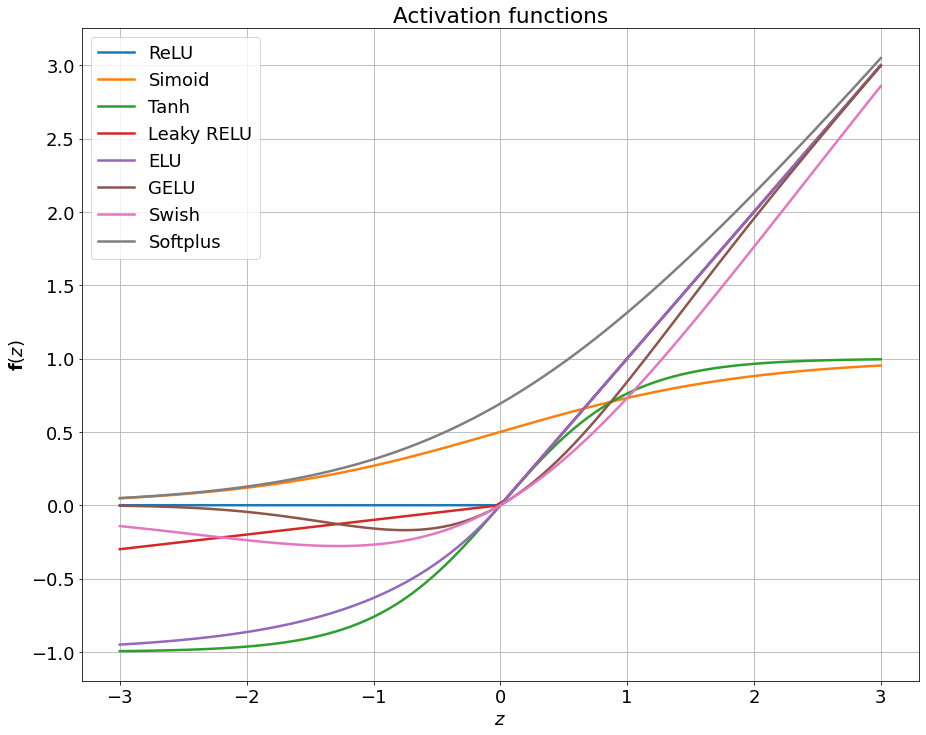
\includegraphics[width=12cm]{activation_functions.png}
  \caption{Activation functions}
\end{figure}

\subsection{Deep Neural Networks}

A deep (feedforward) neural network refers to a neural network that contains not only the input and output layers, but also hidden layers in between. For example, below is a deep feedfoward neural network of 3 hidden layers, with each hidden layer consisting of $d^{(l)}$ units:

\begin{figure}[h!]
  \centering
  \resizebox{11cm}{!}{
    \begin{tikzpicture}[x=2.2cm,y=1.4cm]
      \message{^^JNeural network, shifted}
      \readlist\Nnod{4,5,5,5,3} % array of number of nodes per layer
      \readlist\Nstr{d^{(0)}, d^{(1)}, d^{(2)}, d^{(3)}, d^{(4)}} % array of string number of nodes per layer
      \readlist\Cstr{\strut x,a^{(\prev)},a^{(\prev)},a^{(\prev)},\hat{y}} % array of coefficient symbol per layer
      \def\yshift{0.5} % shift last node for dots
      
      \message{^^J  Layer}
      \foreachitem \N \in \Nnod{ % loop over layers
        \def\lay{\Ncnt} % alias of index of current layer
        \pgfmathsetmacro\prev{int(\Ncnt-1)} % number of previous layer
        \message{\lay,}
        \foreach \i [evaluate={\c=int(\i==\N); \y=\N/2-\i-\c*\yshift;
               \index=(\i<\N?int(\i):"\Nstr[\lay]");
               \x=\lay; \n=\nstyle;}] in {1,...,\N}{ % loop over nodes
        % NODES
        \node[node \n] (N\lay-\i) at (\x,\y) {$\Cstr[\lay]_{\index}$};
        
        % CONNECTIONS
        \ifnum\lay>1 % connect to previous layer
          \foreach \j in {1,...,\Nnod[\prev]}{ % loop over nodes in previous layer
          \draw[connect,white,line width=1.2] (N\prev-\j) -- (N\lay-\i);
          \draw[connect] (N\prev-\j) -- (N\lay-\i);
          %\draw[connect] (N\prev-\j.0) -- (N\lay-\i.180); % connect to left
          }
        \fi % else: nothing to connect first layer
        
        }
        \path (N\lay-\N) --++ (0,1+\yshift) node[midway,scale=1.5] {$\vdots$};
      }
      
      % LABELS
      \node[above=0.5cm,align=center,mygreen!60!black] at (N1-1.90) {input\\[-0.2em]layer};
      \node[above=0.5cm,align=center,myblue!60!black] at (N3-1.90) {hidden layers};
      \node[above=0.5cm,align=center,myred!60!black] at (N\Nnodlen-1.90) {output\\[-0.2em]layer};
      
    \end{tikzpicture}
  }
  \caption{Neural network with 3 hidden layers}
\end{figure}

One of the main advantages of deep neural networks is that in many cases, they can learn to extract very complex and sophisticated features from just the raw features presented to them as their input. For instance, in the context of image recognition, neural networks can extract the features that differentiate a cat from a dog based only on the raw pixel data presented to them from images.

The initial few layers of a neural network typically capture the simpler and smaller features whereas the later layers use information from these low-level features to identify more complex and sophisticated features.

\subsection{The role of backpropagation in training deep neural networks}

In Artificial Neural Networks (ANN), proper training of a neural network is the most important aspect of producing a reliable model. This training is usually associated with the term “Backpropagation”, which is highly vague to most people getting into Deep Learning. Back-propagation is the essence of neural net training. It is the practice of fine-tuning the weights of a neural net based on the error rate (the loss) obtained in the previous epoch (or iteration). Proper tuning of the weights ensures lower error rates after each time of being updated, making the model valid and reliable by increasing its generalization.

\section{Backpropagation Formulations}

\subsection{Notations}
\begin{itemize}
  \item $a$: A scalar
    \item $\bold{a}$: A vector
    \item $\bold{W}$: A matrix
     \item $\bold{W}_{i,:}$: Row $i$ of matrix $\bold{W}$
      \item $\bold{W}_{:,j}$ or $\bold{w}_j$: Column $j$ of matrix $\bold{W}$
       \item $\bold{W^{(l)}}$: weights connect from (l-1)-th layer to l-th layer
      \item $\bold{b}^{(l)}$: bias connect from (l-1)-th layer to l-th layer
      \item $w_{ij}^{(l)}$: weight connects from i-th neuron of (l-1)-th layer to jth neuron lth layer
      \item $z_{i}^{(l)}$: pre-activated output of neuron i-th of l-th layer
      \item $a_{i}^{(l)}$: activated output of neuron i-th of l-th layer
      \item $d^{(l)}$: number of neuron (dimension) of l-th layer
      \item $\bold{z}^{(l)}$: pre-activated output vector of l-th layer. $\bold{z}^{(l)} = \begin{bmatrix} z_1^{(l)} & z_2^{(l)} & \dots & z_{d^{(l)}}^{(l)}\end{bmatrix}^T$
      \item $\bold{a}^{(l)}$: activated output vector of l-th layer. $\bold{a}^{(l)} = \begin{bmatrix} a_1^{(l)} & a_2^{(l)} &\dots & a_{d^{(l)}}^{(l)}\end{bmatrix}^T$
      \item $\mathcal{L}$: loss function
      \item $\odot$: Element-wise product of two vectors
      \item $\bold{x}=\bold{a}^{(0)}$: input of neural network
\end{itemize}

\subsection{Backpropagation}

\begin{algorithm}[h!]
  \caption{Training neural network}
  \hspace*{\algorithmicindent} \textbf{Input:} {A dataset $\mathcal{D}=\Big\lbrace (\bold{x}_1, \bold{y}_1), (\bold{x}_2, \bold{y}_2), \dots, (\bold{x}_S, \bold{y}_S) \Big\rbrace$, a loss function $\mathcal{L}$} \\
  \hspace*{\algorithmicindent} \textbf{Output:} {A neural network with trained weights $\bold{W}$}
  \begin{algorithmic}[1]
    \State{Initialize neural network weights $\bold{W}$ randomly}
    \While{not converged}
      \State{Get training samples from $\mathcal{D}$} (data loading)
      \State{Calculate neural network output and loss function $\mathcal{L}$} (forward pass)
      \State{Calculate partial derivatives of loss funtion with respect to $\bold{W}$}
      \State{Update neural network weights: \begin{equation*}
        \bold{W} \leftarrow \bold{W} - \alpha  \dfrac{\partial \mathcal{L}}{\partial \bold{W}}
      \end{equation*}}
    \EndWhile
    \State \Return $\bold{W}$
  \end{algorithmic}
\end{algorithm}

\begin{itemize}
  \item Problem: But how do we calculate $\dfrac{\partial \mathcal{L}}{\partial \bold{W}}$?
  \item We can calculate $\dfrac{\partial \mathcal{L}}{\partial \bold{W}}$ by a technique called Backpropagation
\end{itemize}

Backpropagation was invented in the 1970s as a general optimization method for performing automatic differentiation of complex nested functions. 
However, it wasn't until 1986, with the publishing of a paper by \cite{rumelhart1986learning}, titled "Learning Representations by Back-Propagating Errors," that the importance of the algorithm was appreciated by the machine learning community at large.

Backpropagation is the essence of neural network training. 
It is the method of fine-tuning the weights of a neural network based on the error rate obtained in the previous epoch (i.e., iteration). 
Proper tuning of the weights allows us to reduce error rates and make the model reliable by increasing its generalization.

Backpropagation in neural network is a short form for “backward propagation of errors.” 
It is a standard method of training artificial neural networks. 
This method helps calculate the gradient of a loss function with respect to all the weights in the network.

The backpropagation algorithm in neural network computes the gradient of the loss function for a single weight by the chain rule. 
It efficiently computes one layer at a time, unlike a native direct computation. 
It computes the gradient, but it does not define how the gradient is used. 
It generalizes the computation in the delta rule.

The "backwards" part of the name stems from the fact that calculation of the gradient proceeds backwards through the network, with the gradient of the final layer of weights being calculated first and the gradient of the first layer of weights being calculated last. 
Partial computations of the gradient from one layer are reused in the computation of the gradient for the previous layer. 
This backwards flow of the error information allows for efficient computation of the gradient at each layer versus the naive approach of calculating the gradient of each layer separately.

Researchers had long been interested in finding a way to train multilayer artificial neural networks that could automatically discover good "internal representations," i.e. features that make learning easier and more accurate. 
Features can be thought of as the stereotypical input to a specific node that activates that node (i.e. causes it to output a positive value near 1). 
Since a node's activation is dependent on its incoming weights and bias, researchers say a node has learned a feature if its weights and bias cause that node to activate when the feature is present in its input.

By the 1980s, hand-engineering features had become the de facto standard in many fields, especially in computer vision, since experts knew from experiments which features (e.g. lines, circles, edges, blobs in computer vision) made learning simpler. 
However, hand-engineering successful features requires a lot of knowledge and practice. More importantly, since it is not automatic, it is usually very slow.

Backpropagation was one of the first methods able to demonstrate that artificial neural networks could learn good internal representations, i.e. their hidden layers learned nontrivial features. 
Experts examining multilayer feedforward networks trained using backpropagation actually found that many nodes learned features similar to those designed by human experts and those found by neuroscientists investigating biological neural networks in mammalian brains (e.g. certain nodes learned to detect edges, while others computed Gabor filters). Even more importantly, because of the efficiency of the algorithm and the fact that domain experts were no longer required to discover appropriate features, backpropagation allowed artificial neural networks to be applied to a much wider field of problems that were previously off-limits due to time and cost constraints.


\begin{itemize}
  \item Backpropagation: Partial derivatives of loss function with respect to outputs of a layer computed by partial derivatives of loss function with respect to outputs of its successive layer
    \item One training step can decompose of 3 stages:
  \begin{itemize}
    \item Foward pass: Compute output of deep neural network and loss function
       \item Backward pass (Backpropagation): Calculate gradient of loss function with respect to weights of layers. Start from top (output) to first (input) layer
        \item Update: Update neural network weights
  \end{itemize}
\end{itemize}

The derivation of the backpropagation algorithm is fairly straightforward. It follows from the use of the chain rule and product rule in differential calculus. 
Application of these rules is dependent on the differentiation of the activation function, one of the reasons the heaviside step function is not used (being discontinuous and thus, non-differentiable).

At the heart of backpropagation is an expression for the partial derivative $\dfrac{\partial \mathcal{L}}{\partial \bold{W}}$ of the loss function $\mathcal{L}$ with respect to any weight $w$ (or bias $b$) in the network. 
The expression tells us how quickly the loss changes when we change the weights and biases. 
And while the expression is somewhat complex, it also has a beauty to it, with each element having a natural, intuitive interpretation. 
And so backpropagation isn't just a fast algorithm for learning. It actually gives us detailed insights into how changing the weights and biases changes the overall behaviour of the network. 
That's well worth studying in detail.

$\bold{W}^{(l)}$: weights of l-th layer
\begin{equation*}
		\bold{W}^{(l)}=\begin{bmatrix} w_{11}^{(l)} & w_{12}^{(l)} & w_{13}^{(l)} & \dots & w_{1d^{(l)}}^{(l)} \\ w_{21}^{(l)} & w_{22}^{(l)} & w_{23}^{(l)} & \dots & w_{2d^{(l)}}^{(l)} \\ \vdots & \thickspace & \thickspace & \thickspace & \vdots \\ w_{d^{(l-1)}1}^{(l)} & w_{d^{(l-1)}2}^{(l)} & w_{d^{(l-1)}3}^{(l)} & \dots & w_{d^{(l-1)}d^{(l)}}^{(l)}\end{bmatrix} \in \mathbb{R}^{d^{(l-1)} \times d^{(l)}}
\end{equation*}

$\bold{b}^{(l)}$: biases of l-th layer
\begin{equation*}
	  \bold{b}^{(l)}=\begin{bmatrix} b_1^{(l)} \\  b_2^{(l)} \\ \vdots \\ b_{d^{(l)}}^{(l)} \end{bmatrix}
\end{equation*}

Let's begin with a notation which lets us refer to weights in the network in an unambiguous way. 
We'll use $w_{ij}^{(l)}$ to denote the weight for the connection from the i-th neuron in the (l-1)th layer to the j-th neuron in the lth layer.

\begin{figure}[h!]
  \centering
  \resizebox{12cm}{!}{
    \begin{tikzpicture}

      \tikzstyle{every node}=[font=\Large]
      
      \node [circle, draw=black!60, fill=blue!30, minimum size=8mm] (bias_l_minus_1) at (0, 0) {1};
      
      \node[circle, draw=black!60, fill=cyan!60, minimum size=10mm, label={[label distance=0.1cm]-120:$z_1^{(l-1)}$}, label={[label distance=0.1cm]-60:$a_1^{(l-1)}$}] (neuron_1_l_minus_1) at (0, -2.5) {};
      
      \node[circle, draw=black!60, fill=cyan!60, minimum size=10mm, label={[label distance=0.1cm]-120:$z_i^{(l-1)}$}, label={[label distance=0.1cm]-60:$a_i^{(l-1)}$}] (neuron_i_l_minus_1) at (0, -7.5) {};
      
      \node[circle, draw=black!60, fill=cyan!60, minimum size=10mm, label={[label distance=0.1cm]-120:$z_{d^{(l-1)}}^{(l-1)}$}, label={[label distance=0.1cm]-60:$a_{d^{(l-1)}}^{(l-1)}$}] (neuron_d_l_minus_1) at (0, -12.5) {};
      
      \path (neuron_1_l_minus_1) --++ (0, -4) node[midway,scale=5] {$\vdots$};
      \path (neuron_i_l_minus_1) --++ (0, -4) node[midway,scale=5] {$\vdots$};
      
      \node [circle, draw=black!60, fill=blue!30, minimum size=8mm] (bias_l) at (6, 0) {1};
      
      
      \node[circle, draw=black!60, fill=cyan!60, minimum size=10mm, label={[label distance=0.1cm]-120:$z_1^{(l)}$}, label={[label distance=0.1cm]-60:$a_1^{(l)}$}] (neuron_1_l) at (6, -2.5) {};
      
      \node[circle, draw=black!60, fill=cyan!60, minimum size=10mm, label={[label distance=0.1cm]-120:$z_2^{(l)}$}, label={[label distance=0.1cm]-60:$a_2^{(l)}$}] (neuron_2_l) at (6, -5) {};
      
      \node[circle, draw=black!60, fill=cyan!60, minimum size=10mm, label={[label distance=0.1cm]-120:$z_j^{(l)}$}, label={[label distance=0.1cm]-60:$a_j^{(l)}$}] (neuron_j_l) at (6, -10) {};
      
      \node[circle, draw=black!60, fill=cyan!60, minimum size=10mm, label={[label distance=0.1cm]-120:$z_{d^{(l)}}^{(l)}$}, label={[label distance=0.1cm]-60:$a_{d^{(l)}}^{(l)}$}] (neuron_d_l) at (6, -15) {};
      
      \path (neuron_2_l) --++ (0, -4.5) node[midway,scale=5] {$\vdots$};
      \path (neuron_j_l) --++ (0, -4.5) node[midway,scale=5] {$\vdots$};
      
      \draw[->] (bias_l_minus_1) -- (neuron_1_l) node[midway,above] {$b_1^{(l)}$};
      \draw[->, dotted] (bias_l_minus_1) -- (neuron_2_l);
      \draw[->, dotted] (bias_l_minus_1) -- (neuron_j_l);
      \draw[->, dotted] (bias_l_minus_1) -- (neuron_d_l);
      
      \draw[->] (neuron_1_l_minus_1) -- (neuron_1_l) node[midway,above] {$w_{11}^{(l)}$};
      \draw[->, dotted] (neuron_1_l_minus_1) -- (neuron_2_l);
      \draw[->, dotted] (neuron_1_l_minus_1) -- (neuron_j_l);
      \draw[->, dotted] (neuron_1_l_minus_1) -- (neuron_d_l);
      
      \draw[->] (neuron_i_l_minus_1) -- (neuron_1_l) node[midway,above=0.2cm] {$w_{i1}^{(l)}$};
      \draw[->] (neuron_i_l_minus_1) -- (neuron_2_l) node[midway,above=0.2cm] {$w_{i2}^{(l)}$};
      \draw[->] (neuron_i_l_minus_1) -- (neuron_j_l) node[midway,above] {$w_{ij}^{(l)}$};
      \draw[->] (neuron_i_l_minus_1) -- (neuron_d_l) node[midway,below=0.2cm] {$w_{id^{(l)}}^{(l)}$};
      
      \draw[->] (neuron_d_l_minus_1) -- (neuron_1_l) node[midway,above] {$w_{d^{(l-1)}1}^{(l)}$};
      \draw[->, dotted] (neuron_d_l_minus_1) -- (neuron_2_l);
      \draw[->, dotted] (neuron_d_l_minus_1) -- (neuron_j_l);
      \draw[->, dotted] (neuron_d_l_minus_1) -- (neuron_d_l);

      \node[above=1,align=center] at (bias_l_minus_1.90) {(l-1)-th layer};
      \node[above=1,align=center] at (bias_l.90) {l-th layer};
      
      \node at (-10, -5) {$\begin{cases} \bold{W}^{(l)}=\begin{bmatrix} w_{11}^{(l)} & w_{12}^{(l)} & w_{13}^{(l)} & \dots & w_{1d^{(l)}}^{(l)} \\ w_{21}^{(l)} & w_{22}^{(l)} & w_{23}^{(l)} & \dots & w_{2d^{(l)}}^{(l)} \\ \vdots & \thickspace & \thickspace & \thickspace & \vdots \\ w_{d^{(l-1)}1}^{(l)} & w_{d^{(l-1)}2}^{(l)} & w_{d^{(l-1)}3}^{(l)} & \dots & w_{d^{(l-1)}d^{(l)}}^{(l)}\end{bmatrix} \in \mathbb{R}^{d^{(l-1)} \times d^{(l)}} \\ \bold{b}^{(l)}=\begin{bmatrix} b_1^{(l)} \\  b_2^{(l)} \\ \vdots \\ b_{d^{(l)}}^{(l)} \end{bmatrix} \in \mathbb{R}^{d^{(l)}} \end{cases}$};
    \end{tikzpicture}
  }
  \caption{2 successive layers visualization}
\end{figure}

This notation is cumbersome at first, and it does take some work to master. 
But with a little effort you'll find the notation becomes easy and natural. 
One quirk of the notation is the ordering of the $i$ and $j$ indices. 

We use a similar notation for the network's biases and activations. 
Explicitly, we use $b_j^{(l)}$ for the bias of the jth neuron in the lth layer. 
And we use $z_j^{(l)}$ for the pre-activated and $a_j^{(l)}$ for the activation of the jth neuron in the lth layer.

With these notations, the activation $a_j^{(l)}$ of the jth neuron in the lth layer is related to the activations in the (l-1)th layer by the equation:
\begin{equation}
	  z_j^{(l)}=\sum_{i=1}^{d^{(l-1)}}w_{ij}^{(l)}a_i^{(l-1)}+b_j^{(l)}=\Big(\bold{W}_{:,j}^{(l)}\Big)^T \bold{a}^{(l-1)} + b_j^{(l)}
\end{equation}

where the sum is over all neurons i in the (l-1)th layer.
To rewrite this expression in a matrix form we define a weight matrix $\bold{W}^{(l)}$ for each layer l. 
The entries of the weight matrix $\bold{W}^{(l)}$ are just the weights connecting to the lth layer of neurons, that is, the entry in the i-th row and jth column is $w_{ij}^{(l)}$. 
Similarly, for each layer l we define a bias vector, $\bold{b}^{(l)}$. 
You can probably guess how this works - the components of the bias vector are just the values $b_j^{(l)}$, one component for each neuron in the lth layer. 
And finally, we define an activation vector $\bold{a}^{(l)}$ whose components are the activations $a_j^{(l)}$.

Activated output of neuron i-th of l-th layer:
\begin{equation}
	  a_j^{(l)} = \bold{f}(z_j^{(l)})
\end{equation}

Pre-activated output in matrix form:
\begin{equation}
	  \bold{z}^{(l)}=\Big(\bold{W}^{(l)}\Big)^T\bold{a}^{(l-1)} + \bold{b}^{(l)}, l=1, \dots, L
\end{equation}

Activated output in matrix form:
\begin{equation}
	  \bold{a}^{(l)}=\bold{f}(\bold{z}^{(l)}), l=1, \dots, L
\end{equation}

\begin{figure}[h!]
  \centering
  \resizebox{12cm}{!}{
    \begin{tikzpicture}

      \tikzstyle{every node}=[font=\Large]
      \node [circle, draw=black!60, fill=blue!30, minimum size=8mm] (bias_l_minus_1) at (0, 0) {1};
      
      \node[circle, draw=black!60, fill=cyan!60, minimum size=10mm, label={[label distance=0.1cm]-120:$z_1^{(l-1)}$}, label={[label distance=0.1cm]-60:$a_1^{(l-1)}$}] (neuron_1_l_minus_1) at (0, -2.5) {};
      
      \node[circle, draw=black!60, fill=cyan!60, minimum size=10mm, label={[label distance=0.1cm]-120:$z_i^{(l-1)}$}, label={[label distance=0.1cm]-60:$a_i^{(l-1)}$}] (neuron_i_l_minus_1) at (0, -7.5) {};
      
      \node[circle, draw=black!60, fill=cyan!60, minimum size=10mm, label={[label distance=0.1cm]-120:$z_{d^{(l-1)}}^{(l-1)}$}, label={[label distance=0.1cm]-60:$a_{d^{(l-1)}}^{(l-1)}$}] (neuron_d_l_minus_1) at (0, -12.5) {};
      
      \path (neuron_1_l_minus_1) --++ (0, -4) node[midway,scale=5] {$\vdots$};
      \path (neuron_i_l_minus_1) --++ (0, -4) node[midway,scale=5] {$\vdots$};
      
      \node [circle, draw=black!60, fill=blue!30, minimum size=8mm] (bias_l) at (6, 0) {1};
      
      
      \node[circle, draw=black!60, fill=cyan!60, minimum size=10mm, label={[label distance=0.1cm]-120:$z_1^{(l)}$}, label={[label distance=0.1cm]-60:$a_1^{(l)}$}] (neuron_1_l) at (6, -2.5) {};
      
      \node[circle, draw=black!60, fill=cyan!60, minimum size=10mm, label={[label distance=0.1cm]-120:$z_j^{(l)}$}, label={[label distance=0.1cm]-60:$a_j^{(l)}$}] (neuron_j_l) at (6, -9) {};
      
      \node[circle, draw=black!60, fill=cyan!60, minimum size=10mm, label={[label distance=0.1cm]-120:$z_{d^{(l)}}^{(l)}$}, label={[label distance=0.1cm]-60:$a_{d^{(l)}}^{(l)}$}] (neuron_d_l) at (6, -14) {};
      
      \path (neuron_1_l) --++ (0, -4.5) node[midway,scale=5] {$\vdots$};
      \path (neuron_j_l) --++ (0, -4.5) node[midway,scale=5] {$\vdots$};
      
      \node [circle, draw=black!60, fill=blue!30, minimum size=8mm] (bias_l_plus_1) at (12, 0) {1};
      
      
      \node[circle, draw=black!60, fill=cyan!60, minimum size=10mm, label={[label distance=0.1cm]-120:$z_1^{(l+1)}$}, label={[label distance=0.1cm]-60:$a_1^{(l+1)}$}] (neuron_1_l_plus_1) at (12, -2.5) {};
      
      \node[circle, draw=black!60, fill=cyan!60, minimum size=10mm, label={[label distance=0.1cm]-120:$z_k^{(l)}$}, label={[label distance=0.1cm]-60:$a_k^{(l)}$}] (neuron_k_l_plus_1) at (12, -7) {};
      
      \node[circle, draw=black!60, fill=cyan!60, minimum size=10mm, label={[label distance=0.1cm]-120:$z_{d^{(l+1)}}^{(l+1)}$}, label={[label distance=0.1cm]-60:$a_{d^{(l+1)}}^{(l+1)}$}] (neuron_d_l_plus_1) at (12, -11.5) {};
      
      \path (neuron_1_l_plus_1) --++ (0, -3.0) node[midway,scale=5] {$\vdots$};
      \path (neuron_k_l_plus_1) --++ (0, -3.0) node[midway,scale=5] {$\vdots$};
      
      \draw[->] (bias_l_minus_1) -- (neuron_1_l) node[midway,above] {$b_1^{(l)}$};
      \draw[->, dotted] (bias_l_minus_1) -- (neuron_j_l);
      \draw[->, dotted] (bias_l_minus_1) -- (neuron_d_l);
      
      \draw[->, dotted] (neuron_1_l_minus_1) -- (neuron_1_l);
      \draw[->, dotted] (neuron_1_l_minus_1) -- (neuron_j_l);
      \draw[->, dotted] (neuron_1_l_minus_1) -- (neuron_d_l);
      
      \draw[->] (neuron_i_l_minus_1) -- (neuron_1_l) node[midway,above=0.2cm] {$w_{i1}^{(l)}$};
      \draw[->] (neuron_i_l_minus_1) -- (neuron_j_l) node[midway,above] {$w_{ij}^{(l)}$};
      \draw[->] (neuron_i_l_minus_1) -- (neuron_d_l) node[midway,below=0.2cm] {$w_{id^{(l)}}^{(l)}$};
      
      \draw[->, dotted] (neuron_d_l_minus_1) -- (neuron_1_l);
      \draw[->, dotted] (neuron_d_l_minus_1) -- (neuron_j_l);
      \draw[->, dotted] (neuron_d_l_minus_1) -- (neuron_d_l);
      
      \draw[->, dotted] (bias_l) -- (neuron_1_l_plus_1);
      \draw[->] (bias_l) -- (neuron_k_l_plus_1) node[midway, above=0.5cm] {$b_{k}^{(l+1)}$};
      \draw[->, dotted] (bias_l) -- (neuron_d_l_plus_1);
      
      \draw[->, dotted] (neuron_1_l) -- (neuron_1_l_plus_1);
      \draw[->] (neuron_1_l) -- (neuron_k_l_plus_1) node[midway, below=0.25cm] {$w_{1k}^{(l+1)}$};
      \draw[->, dotted] (neuron_1_l) -- (neuron_d_l_plus_1);
      
      \draw[->, dotted] (neuron_j_l) -- (neuron_1_l_plus_1);
      \draw[->] (neuron_j_l) -- (neuron_k_l_plus_1) node[midway, above=0.25cm] {$w_{jk}^{(l+1)}$};
      \draw[->, dotted] (neuron_j_l) -- (neuron_d_l_plus_1);
      
      \draw[->, dotted] (neuron_d_l) -- (neuron_1_l_plus_1);
      \draw[->] (neuron_d_l) -- (neuron_k_l_plus_1) node[midway, above=0.5cm] {$w_{d^{(l)}k}^{(l+1)}$};
      \draw[->, dotted] (neuron_d_l) -- (neuron_d_l_plus_1);
      
      \node[above=1,align=center] at (bias_l_minus_1.90) {(l-1)-th layer};
      \node[above=1,align=center] at (bias_l.90) {l-th layer};
      \node[above=1,align=center] at (bias_l_plus_1.90) {(l+1)-th layer};
      
      \node[below=2, align=center] at (neuron_d_l_minus_1.-90) {$\mathbf{z}^{(l-1)}-\mathbf{a}^{(l-1)}$};
      
      \node[below=2, align=center] at (neuron_d_l.-90) {$\mathbf{z}^{(l)}-\mathbf{a}^{(l)}$};
      
      \node[below=2, align=center] at (neuron_d_l_plus_1.-90) {$\mathbf{z}^{(l+1)}-\mathbf{a}^{(l+1)}$};
      
      \node at (-5, 0) {$\begin{cases}\mathbf{W}^{(l)} \in \mathbb{R}^{d^{(l)}\times d^{(l+1)}} \\ \mathbf{b}^{(l)} \in \mathbb{R}^{d^{(l)}} \end{cases}$};
      
      \node at (-5, -3) {$\begin{aligned}z_j^{(l)}&=\displaystyle\sum_{i=1}^{d^{(l-1)}}w_{ij}^{(l)}a_i^{(l-1)}+b_j^{(l)}\\&=\Big(\bold{W}_{:,j}^{(l)}\Big)^T \bold{a}^{(l-1)} + b_j^{(l)}\end{aligned}$};
      
      \node at (-5, -5) {$\bold{z}^{(l)}=\Big(\bold{W}^{(l)}\Big)^T\bold{a}^{(l-1)} + \bold{b}^{(l)}$};
      
      \node at (-5, -8) {$\begin{aligned} a_j^{(l)} &= \mathbf{f} \big( z_i^{(l)} \big)\\&=\mathbf{f} \Big(\displaystyle\sum_{i=1}^{d^{(l-1)}}w_{ij}^{(l)}a_i^{(l-1)}+b_j^{(l)} \Big) \\&= \mathbf{f} \Big\lbrack \Big(\bold{W}_{:,j}^{(l)}\Big)^T \bold{a}^{(l-1)} + b_j^{(l)} \Big\rbrack \end{aligned}$};
      
      \node at (-5, -12) {$\begin{aligned} \mathbf{a}^{(l)}&=\mathbf{f} \Big( \mathbf{z}^{(l)} \Big)\\&=\mathbf{f} \Big\lbrack\Big(\bold{W}^{(l)}\Big)^T\bold{a}^{(l-1)} + \bold{b}^{(l)} \Big\rbrack \end{aligned}$};
    \end{tikzpicture}
  }
  \caption{3 layers visualization}
\end{figure}

When we need to compute $\bold{a}^{(l)}$, we compute the intermediate quantity $\bold{z}^{(l)}=\Big(\bold{W}^{(l)}\Big)^T\bold{a}^{(l-1)} + \bold{b}^{(l)}$ is the pre-activated output of j-th neuron of l-th layer.
This quantity turns out to be useful enough to be worth naming: we call $\bold{z}^{(l)}$ the weighted input to the neurons in layer l. 
We'll make considerable use of the weighted input $\bold{z}^{(l)}$ or pre-activated output.
It's also worth noting that $\bold{z}^{(l)}$ has components $\bold{z}_j^{(l)}$, that is, $\bold{z}_j^{(l)}$ is just the weighted input to the activation function for neuron j in layer l.

Loss function:
\begin{equation}
	  \mathcal{L} = \ell\Big(\bold{a}^{(L)}, \bold{y} \Big)
\end{equation}

Backpropagation is about understanding how changing the weights and biases in a network changes the cost function. 
Ultimately, this means computing the partial derivatives $\dfrac{\partial \mathcal{L}}{\partial w_{ij}^{(l)}}$ and $\dfrac{\partial \mathcal{L}}{\partial b_{j}^{(l)}}$. 
But to compute those, we first introduce an intermediate quantity, $e_j^{(l)}$, which we call the error in the jth neuron in the lth layer. 
Backpropagation will give us a procedure to compute the error $e_j^{(l)}$, and then will relate $e_j^{(l)}$ to $\dfrac{\partial \mathcal{L}}{\partial w_{ij}^{(l)}}$ and $\dfrac{\partial \mathcal{L}}{\partial b_{j}^{(l)}}$.

We need to calculate partial derivatives of $\mathcal{L}$ with respect to all $\bold{W}^{(l)}$ and $\bold{b}^{(l)}, l=1, \dots, L$.
The derivation of the backpropagation algorithm begins by applying the chain rule to the error function partial derivative

\begin{equation}
  \dfrac{\partial \mathcal{L}}{w_{ij}^{(l)}}=\dfrac{\partial \mathcal{L}}{\partial z_{j}^{(l)}}\dfrac{\partial z_j^{(l)}}{w_{ij}^{(l)}}=\dfrac{\partial \mathcal{L}}{\partial z_{j}^{(l)}}a_i^{(l-1)}
\end{equation}

\begin{equation}
  \dfrac{\partial \mathcal{L}}{\partial b_j^{(l)}}=\dfrac{\partial \mathcal{L}}{\partial z_{j}^{(l)}}\dfrac{\partial z_j^{(l)}}{\partial b_j^{(l)}}=\dfrac{\partial \mathcal{L}}{\partial z_{j}^{(l)}}
\end{equation}

We set:
\begin{equation}
	  \dfrac{\partial \mathcal{L}}{\partial z_{j}^{(l)}}:=e_j^{(l)}
\end{equation}

At output layer ($L$-th layer):

\begin{equation}
	\begin{aligned}
		\dfrac{\partial \mathcal{L}}{w_{ij}^{(L)}}&=\dfrac{\partial \mathcal{L}}{\partial z_{j}^{(L)}}\dfrac{\partial z_j^{(L)}}{w_{ij}^{(L)}}\\&=\dfrac{\partial \mathcal{L}}{\partial z_{j}^{(L)}}a_i^{(L-1)}\\&=\dfrac{\partial\mathcal{L}}{\partial a_j^{(L)}}\dfrac{\partial a_j^{(L)}}{\partial z_j^{(L)}}a_i^{(L-1)}\\&=\dfrac{\partial\mathcal{L}}{\partial a_j^{(L)}}\bold{f}^{\prime}\Big(z_j^{(L)}\Big)a_i^{(L-1)}
	\end{aligned}
\end{equation}

\begin{equation}
	\begin{aligned}
		\bold{e}^{(L)}&=\begin{bmatrix} \dfrac{\partial\mathcal{L}}{\partial z_1^{(L)}} & \dfrac{\partial\mathcal{L}}{\partial z_2^{(L)}} & \dots & \dfrac{\partial\mathcal{L}}{\partial z_{d^{(L)}}^{(L)}} \end{bmatrix}^T\\&=\begin{bmatrix} \dfrac{\partial\mathcal{L}}{\partial a_1^{(L)}}\dfrac{\partial a_1^{(L)}}{\partial z_1^{(L)}} & \dfrac{\partial\mathcal{L}}{\partial a_2^{(L)}}\dfrac{\partial a_2^{(L)}}{\partial z_2^{(L)}} & \dots & \dfrac{\partial\mathcal{L}}{\partial a_{d^{(L)}}^{(L)}}\dfrac{\partial a_{d^{(L)}}^{(L)}}{\partial z_{d^{(L)}}^{(L)}} \end{bmatrix}^T\\&=\begin{bmatrix} \dfrac{\partial\mathcal{L}}{\partial a_1^{(L)}}\bold{f}^{\prime}\Big(z_1^{(L)}\Big) & \dfrac{\partial\mathcal{L}}{\partial a_2^{(L)}}\bold{f}^{\prime}\Big(z_2^{(L)}\Big) & \dots & \dfrac{\partial\mathcal{L}}{\partial a_{d^{(L)}}^{(L)}}\bold{f}^{\prime}\Big(z_{d^{(L)}}^{(L)}\Big) \end{bmatrix}^T\\&=\dfrac{\partial \mathcal{L}}{\partial \bold{a}^{(L)}} \odot \bold{f}^{\prime}(\bold{z}^{(L)})
	\end{aligned}
\end{equation}

\begin{equation}
	\Rightarrow \begin{cases}\dfrac{\partial \mathcal{L}}{\partial \bold{W}^{(L)}}=\bold{a}^{(L-1)}\Big(\bold{e}^{(L)}\Big)^T \\ \dfrac{\partial \mathcal{L}}{\partial \bold{b}^{(L)}}=\bold{e}^{(L)} \end{cases}
\end{equation}

\begin{figure}[h!]
  \centering
  \resizebox{15.0cm}{!}{
    \begin{tikzpicture}

      \tikzstyle{every node}=[font=\Large]
      
      \node [circle, draw=black!60, fill=blue!30, minimum size=8mm] (bias_l_minus_1) at (0, 0) {1};
      
      \node[circle, draw=black!60, fill=cyan!60, minimum size=10mm, label={[label distance=0.1cm]-120:$z_1^{(L-1)}$}, label={[label distance=0.1cm]-60:$a_1^{(L-1)}$}] (neuron_1_l_minus_1) at (0, -2.5) {};
      
      \node[circle, draw=black!60, fill=cyan!60, minimum size=10mm, label={[label distance=0.1cm]-120:$z_i^{(L-1)}$}, label={[label distance=0.1cm]-60:$a_i^{(L-1)}$}] (neuron_i_l_minus_1) at (0, -7.5) {};
      
      \node[circle, draw=black!60, fill=cyan!60, minimum size=10mm, label={[label distance=0.1cm]-120:$z_{d^{(L-1)}}^{(l-1)}$}, label={[label distance=0.1cm]-60:$a_{d^{(L-1)}}^{(l-1)}$}] (neuron_d_l_minus_1) at (0, -12.5) {};
      
      \path (neuron_1_l_minus_1) --++ (0, -4) node[midway,scale=5] {$\vdots$};
      \path (neuron_i_l_minus_1) --++ (0, -4) node[midway,scale=5] {$\vdots$};
      
      
      \node[circle, draw=black!60, fill=cyan!60, minimum size=10mm, label={[label distance=0.1cm]-120:$z_1^{(L)}$}, label={[label distance=0.1cm]-60:$a_1^{(L)}$}] (neuron_1_l) at (6, -2.5) {};
      
      \node[circle, draw=black!60, fill=cyan!60, minimum size=10mm, label={[label distance=0.1cm]-120:$z_2^{(L)}$}, label={[label distance=0.1cm]-60:$a_2^{(L)}$}] (neuron_2_l) at (6, -5) {};
      
      \node[circle, draw=black!60, fill=cyan!60, minimum size=10mm, label={[label distance=0.1cm]-120:$z_j^{(L)}$}, label={[label distance=0.1cm]-60:$a_j^{(L)}$}] (neuron_j_l) at (6, -10) {};
      
      \node[circle, draw=black!60, fill=cyan!60, minimum size=10mm, label={[label distance=0.1cm]-120:$z_{d^{(L)}}^{(L)}$}, label={[label distance=0.1cm]-60:$a_{d^{(L)}}^{(L)}$}] (neuron_d_l) at (6, -15) {};
      
      \path (neuron_2_l) --++ (0, -4.5) node[midway,scale=5] {$\vdots$};
      \path (neuron_j_l) --++ (0, -4.5) node[midway,scale=5] {$\vdots$};
      
      \node[rectangle, draw=red!60, minimum size = 20mm, color=red] (loss) at (15, -7.5) {$\begin{aligned}\mathcal{L}&=\ell \Big(a_1^{(L)}, a_2^{(L)}, \dots, a_{d^{(L)}}^{(L)}, \bold{y} \Big) \\&= \ell \Big( \mathbf{a}^{(L)}, \bold{y} \Big) \end{aligned}$};
      
      \draw[->] (bias_l_minus_1) -- (neuron_1_l) node[midway,above] {$b_1^{(L)}$};
      \draw[->, dotted] (bias_l_minus_1) -- (neuron_2_l);
      \draw[->, dotted] (bias_l_minus_1) -- (neuron_j_l);
      \draw[->, dotted] (bias_l_minus_1) -- (neuron_d_l);
      
      \draw[->] (neuron_1_l_minus_1) -- (neuron_1_l) node[midway,above] {$w_{11}^{(L)}$};
      \draw[->, dotted] (neuron_1_l_minus_1) -- (neuron_2_l);
      \draw[->, dotted] (neuron_1_l_minus_1) -- (neuron_j_l);
      \draw[->, dotted] (neuron_1_l_minus_1) -- (neuron_d_l);
      
      \draw[->] (neuron_i_l_minus_1) -- (neuron_1_l) node[midway,above=0.2cm] {$w_{i1}^{(L)}$};
      \draw[->] (neuron_i_l_minus_1) -- (neuron_2_l) node[midway,above=0.2cm] {$w_{i2}^{(L)}$};
      \draw[->] (neuron_i_l_minus_1) -- (neuron_j_l) node[midway,above] {$w_{ij}^{(L)}$};
      \draw[->] (neuron_i_l_minus_1) -- (neuron_d_l) node[midway,below=0.2cm] {$w_{id^{(L)}}^{(L)}$};
      
      \draw[->] (neuron_d_l_minus_1) -- (neuron_1_l) node[midway,above] {$w_{d^{(L-1)}1}^{(L)}$};
      \draw[->, dotted] (neuron_d_l_minus_1) -- (neuron_2_l);
      \draw[->, dotted] (neuron_d_l_minus_1) -- (neuron_j_l);
      \draw[->, dotted] (neuron_d_l_minus_1) -- (neuron_d_l);
      
      \draw[->, draw=red] (loss.west) -- (neuron_1_l) node[color=red, midway, above] {$e_1^{(L)}$};
      \draw[->, draw=red] (loss.west) -- (neuron_2_l) node[color=red, midway, below=0.25cm] {$e_2^{(L)}$};
      \draw[->, draw=red] (loss.west) -- (neuron_j_l) node[color=red, midway, above] {$e_j^{(L)}$};
      \draw[->, draw=red] (loss.west) -- (neuron_d_l) node[color=red, midway, below=0.25cm] {$e_{d^{(L)}}^{(L)}$};
      
      \node[above=1,align=center] at (bias_l_minus_1.90) {(L-1)-th layer};
      \node[above=1,align=center] at (bias_l.90) {L-th layer (Output layer)};

      \node at (-10, -5) {$\begin{cases}
            \dfrac{\partial \mathcal{L}}{w_{ij}^{(L)}}=\dfrac{\partial \mathcal{L}}{\partial z_{j}^{(L)}}\dfrac{\partial z_j^{(L)}}{w_{ij}^{(L)}}=\dfrac{\partial \mathcal{L}}{\partial z_{j}^{(L)}}a_i^{(L-1)}=a_i^{(L-1)}\dfrac{\partial \mathcal{L}}{\partial z_{j}^{(L)}}=a_i^{(L-1)}e_j^{(L)}\\
            \dfrac{\partial \mathcal{L}}{\partial b_j^{(L)}}=\dfrac{\partial \mathcal{L}}{\partial z_{j}^{(L)}}\dfrac{\partial z_j^{(L)}}{\partial b_j^{(L)}}=\dfrac{\partial \mathcal{L}}{\partial z_{j}^{(L)}}=e_j^{(L)}
          \end{cases}$};
          
      \node at (-10, -9) {$\begin{aligned}
            \bold{e}^{(L)}&=\begin{bmatrix} \dfrac{\partial\mathcal{L}}{\partial z_1^{(L)}} & \dfrac{\partial\mathcal{L}}{\partial z_2^{(L)}} & \dots & \dfrac{\partial\mathcal{L}}{\partial z_{d^{(L)}}^{(L)}} \end{bmatrix}^T\\&=\begin{bmatrix} e_1^{(L)} & e_2^{(L)} & \dots & e_{d^{(L)}}^{(L)} \end{bmatrix}^T
          \end{aligned}$};
          
      \node at (-10, -12) {$\Rightarrow\begin{cases}\dfrac{\partial \mathcal{L}}{\partial \bold{W}^{(L)}}=\bold{a}^{(L-1)}\Big(\bold{e}^{(L)}\Big)^T \\ \dfrac{\partial \mathcal{L}}{\partial \bold{b}^{(L)}}=\bold{e}^{(L)} \end{cases}$};
      
    \end{tikzpicture}
  }
  \caption{Backpropagation visualization at output layer}
\end{figure}

At l-th layer ($1 \leq l < L$):

\begin{equation}
	\dfrac{\partial \mathcal{L}}{\partial w_{ij}^{(l)}}=\dfrac{\partial \mathcal{L}}{\partial z_j^{(l)}}\dfrac{\partial z_j^{(l)}}{\partial w_{ij}^{(l)}}=\dfrac{\partial \mathcal{L}}{\partial z_j^{(l)}} a_i^{(l-1)}=e_j^{(l)}a_i^{(l-1)}
\end{equation}

\begin{equation}
	\dfrac{\partial \mathcal{L}}{\partial b_j^{(l)}}=\dfrac{\partial \mathcal{L}}{\partial z_j^{(l)}}\dfrac{\partial z_j^{(l)}}{\partial b_j^{(l)}}=\dfrac{\partial \mathcal{L}}{\partial z_j^{(l)}} = e_j^{(l)}
\end{equation}

\begin{equation}
	\Rightarrow \begin{cases} \dfrac{\partial \mathcal{L}}{\partial \bold{W}^{(l)}}=\bold{a}^{(l-1)}\Big(\bold{e}^{(l)}\Big)^T \\ \dfrac{\partial \mathcal{L}}{\partial \bold{b}^{(l)}}=\bold{e}^{(l)} \end{cases}
\end{equation}

Now the question arises of how to calculate the partial derivatives of layers other than the output layer. Fortunately, the chain rule for multivariate functions comes to the rescue again. Observe the following equation for the error term $e_j^{(l)}$.
We consider $\mathcal{L} = \mathcal{L}\Big(\bold{z}^{(l+1)}\Big)=\mathcal{L}\Big(z_1^{(l+1)}, z_2^{(l+1)}, \dots, z_{d^{(l+1)}}^{(l+1)}\Big)$:
\begin{equation}
	\begin{aligned}
		\dfrac{\partial \mathcal{L}}{\partial z_j^{(l)}}&=\sum_{k=1}^{d^{(l+1)}}\dfrac{\partial \mathcal{L}}{\partial z_k^{(l+1)}} \dfrac{\partial z_k^{(l+1)}}{\partial z_j^{(l)}}\\&=\sum_{k=1}^{d^{(l+1)}} \dfrac{\partial \mathcal{L}}{\partial z_k^{(l+1)}} \dfrac{\partial z_k^{(l+1)}}{\partial a_j^{(l)}} \dfrac{\partial a_j^{(l)}}{\partial z_j^{(l)}}\\&=\sum_{k=1}^{d^{(l+1)}}\dfrac{\partial \mathcal{L}}{\partial z_k^{(l+1)}}w_{jk}^{(l+1)}\bold{f}^{\prime}\Big(z_j^{(l)}\Big)
	\end{aligned}
\end{equation}

\begin{equation}
	\begin{aligned}
		e_j^{(l)}&=\dfrac{\partial \mathcal{L}}{\partial z_j^{(l)}}\\&=\sum_{k=1}^{d^{(l+1)}}e_k^{(l+1)}w_{jk}^{(l+1)}\bold{f}^{\prime}\Big(z_j^{(l)}\Big)\\&=\bold{f}^{\prime}(z_j^{(l)})\bold{W}_{j,:}^{(l+1)}\bold{e}^{(l+1)}
	\end{aligned}
\end{equation}

In matrix form:

\begin{equation}
  \bold{e}^{(l)}=\bold{W}^{(l+1)}\bold{e}^{(l+1)}\odot\bold{f}^{\prime}(\bold{z}^{(l)})
\end{equation}

This equation is where backpropagation gets its name. 
Namely, the error $\bold{e}^{(l)}$ is dependent on the errors $\bold{e}^{(l+1)}$.
Thus, errors flow backward, from the last layer to the first layer. 
All that is needed is to compute the first error terms based on the computed output $\hat{\bold{y}}$ and the target output $\bold{y}$.
Then, the error terms for the previous layer are computed by performing a product sum (weighted by $w_{jk}^{(l+1)}$) of the error terms for the next layer and scaling by $\bold{f}^{\prime}(z_j^{(l)})$, repeated until the input layer is reached.


This backwards propagation of errors is very similar to the forward computation that calculates the neural network's output. Thus, calculating the output is often called the forward pass while calculating the error terms and derivatives is often called the backward pass.
While going in the forward direction, the inputs are repeatedly recombined from the first layer to the last by product sums dependent on the weights $w_{ij}^{(l)}$.
In the backward direction, the "inputs" are the final layer's error terms, which are repeatedly recombined from the last layer to the first by product sums dependent on the weights $w_{jk}^{(l+1)}$.

\begin{figure}[h!]
  \centering
  \resizebox{15cm}{!}{
    \begin{tikzpicture}

      \tikzstyle{every node}=[font=\Large]
      
      \node [circle, draw=black!60, fill=blue!30, minimum size=8mm] (bias_l_minus_1) at (0, 0) {1};
      
      \node[circle, draw=black!60, fill=cyan!60, minimum size=10mm, label={[label distance=0.1cm]-120:$z_1^{(l-1)}$}, label={[label distance=0.1cm]-60:$a_1^{(l-1)}$}] (neuron_1_l_minus_1) at (0, -2.5) {};
      
      \node[circle, draw=black!60, fill=cyan!60, minimum size=10mm, label={[label distance=0.1cm]-120:$z_i^{(l-1)}$}, label={[label distance=0.1cm]-60:$a_i^{(l-1)}$}] (neuron_i_l_minus_1) at (0, -7.5) {};
      
      \node[circle, draw=black!60, fill=cyan!60, minimum size=10mm, label={[label distance=0.1cm]-120:$z_{d^{(l-1)}}^{(l-1)}$}, label={[label distance=0.1cm]-60:$a_{d^{(l-1)}}^{(l-1)}$}] (neuron_d_l_minus_1) at (0, -12.5) {};
      
      \path (neuron_1_l_minus_1) --++ (0, -4) node[midway,scale=5] {$\vdots$};
      \path (neuron_i_l_minus_1) --++ (0, -4) node[midway,scale=5] {$\vdots$};
      
      \node [circle, draw=black!60, fill=blue!30, minimum size=8mm] (bias_l) at (6, 0) {1};
      
      
      \node[circle, draw=black!60, fill=cyan!60, minimum size=10mm, label={[label distance=0.1cm]-120:$z_1^{(l)}$}, label={[label distance=0.1cm]-60:$a_1^{(l)}$}] (neuron_1_l) at (6, -2.5) {};
      
      \node[circle, draw=black!60, fill=cyan!60, minimum size=10mm, label={[label distance=0.1cm]-120:$z_j^{(l)}$}, label={[label distance=0.1cm]-60:$a_j^{(l)}$}] (neuron_j_l) at (6, -9) {};
      
      \node[circle, draw=black!60, fill=cyan!60, minimum size=10mm, label={[label distance=0.1cm]-120:$z_{d^{(l)}}^{(l)}$}, label={[label distance=0.1cm]-60:$a_{d^{(l)}}^{(l)}$}] (neuron_d_l) at (6, -14) {};
      
      \path (neuron_1_l) --++ (0, -4.5) node[midway,scale=5] {$\vdots$};
      \path (neuron_j_l) --++ (0, -4.5) node[midway,scale=5] {$\vdots$};
      
      
      \node[circle, draw=black!60, fill=cyan!60, minimum size=10mm, label={[label distance=0.1cm]-120:$z_1^{(l+1)}$}, label={[label distance=0.1cm]-60:$a_1^{(l+1)}$}] (neuron_1_l_plus_1) at (12, -2.5) {};
      
      \node[circle, draw=black!60, fill=cyan!60, minimum size=10mm, label={[label distance=0.1cm]-120:$z_k^{(l)}$}, label={[label distance=0.1cm]-60:$a_k^{(l)}$}] (neuron_k_l_plus_1) at (12, -7) {};
      
      \node[circle, draw=black!60, fill=cyan!60, minimum size=10mm, label={[label distance=0.1cm]-120:$z_{d^{(l+1)}}^{(l+1)}$}, label={[label distance=0.1cm]-60:$a_{d^{(l+1)}}^{(l+1)}$}] (neuron_d_l_plus_1) at (12, -11.5) {};
      
      \path (neuron_1_l_plus_1) --++ (0, -3.0) node[midway,scale=5] {$\vdots$};
      \path (neuron_k_l_plus_1) --++ (0, -3.0) node[midway,scale=5] {$\vdots$};
      
      \node [circle, draw=black!60, fill=blue!30, minimum size=8mm] (bias_l_plus_1) at (12, 0) {1};
      
      \draw[->] (bias_l_minus_1) -- (neuron_1_l) node[midway,above] {$b_1^{(l)}$};
      \draw[->, dotted] (bias_l_minus_1) -- (neuron_j_l);
      \draw[->, dotted] (bias_l_minus_1) -- (neuron_d_l);
      
      \draw[->, dotted] (neuron_1_l_minus_1) -- (neuron_1_l);
      \draw[->, dotted] (neuron_1_l_minus_1) -- (neuron_j_l);
      \draw[->, dotted] (neuron_1_l_minus_1) -- (neuron_d_l);
      
      \draw[->] (neuron_i_l_minus_1) -- (neuron_1_l) node[midway,above=0.2cm] {$w_{i1}^{(l)}$};
      \draw[->] (neuron_i_l_minus_1) -- (neuron_j_l) node[midway,above] {$w_{ij}^{(l)}$};
      \draw[->] (neuron_i_l_minus_1) -- (neuron_d_l) node[midway,below=0.2cm] {$w_{id^{(l)}}^{(l)}$};
      
      \draw[->, dotted] (neuron_d_l_minus_1) -- (neuron_1_l);
      \draw[->, dotted] (neuron_d_l_minus_1) -- (neuron_j_l);
      \draw[->, dotted] (neuron_d_l_minus_1) -- (neuron_d_l);
      
      \draw[->, color=red] (neuron_1_l_plus_1) -- (bias_l)  node[midway, above=0.5cm] {$e_{1}^{(l+1)}$};
      \draw[->, color=red] (neuron_k_l_plus_1) -- (bias_l)  node[midway, above=0.5cm] {$e_{k}^{(l+1)}$};
      \draw[->, dotted, color=red] (neuron_d_l_plus_1) -- (bias_l);
      
      \draw[->, dotted, color=red] (neuron_1_l_plus_1) -- (neuron_1_l);
      \draw[->, dotted, color=red] (neuron_k_l_plus_1) -- (neuron_1_l);
      \draw[->, dotted, color=red] (neuron_d_l_plus_1) -- (neuron_1_l);
      
      \draw[->, color=red] (neuron_1_l_plus_1) -- (neuron_j_l)node[midway, above=0.25cm] {$w_{j1}^{(l+1)}e_1^{(l+1)}$};
      \draw[->, color=red] (neuron_k_l_plus_1) -- (neuron_j_l)  node[midway, above=0.25cm] {$w_{jk}^{(l+1)}e_k^{(l+1)}$};
      \draw[->, color=red] (neuron_d_l_plus_1) -- (neuron_j_l) node[midway, above=0.25cm] {$w_{jd^{(l+1)}}^{(l+1)}e_{jd^{(l+1)}}^{(l+1)}$};
      
      \draw[->, dotted, color=red] (neuron_1_l_plus_1) -- (neuron_d_l);
      \draw[->, dotted, color=red] (neuron_k_l_plus_1) -- (neuron_d_l);
      \draw[->, dotted, color=red] (neuron_d_l_plus_1) -- (neuron_d_l);
      
      \node[above=1,align=center] at (bias_l_minus_1.90) {(l-1)-th layer};
      \node[above=1,align=center] at (bias_l.90) {l-th layer};
      \node[above=1,align=center] at (bias_l_plus_1.90) {(l+1)-th layer};
      
      \node[below=2, align=center] at (neuron_d_l_minus_1.-90) {$\mathbf{z}^{(l-1)}-\mathbf{a}^{(l-1)}$};
      
      \node[below=2, align=center] at (neuron_d_l.-90) {$\mathbf{z}^{(l)}-\mathbf{a}^{(l)}$};
      
      \node[below=2, align=center] at (neuron_d_l_plus_1.-90) {$\mathbf{z}^{(l+1)}-\mathbf{a}^{(l+1)}$};
      
      \node at (-10, -3) {$\begin{aligned}
            e_j^{(l)}&=\dfrac{\partial \mathcal{L}}{\partial z_j^{(l)}}\\&=\sum_{k=1}^{d^{(l+1)}}e_k^{(l+1)}w_{jk}^{(l+1)}\bold{f}^{\prime}\Big(z_j^{(l)}\Big)\\&=\bold{f}^{\prime}(z_j^{(l)})\bold{W}_{j,:}^{(l+1)}\bold{e}^{(l+1)}
            \end{aligned}$};
            
      \node at (-10, -6) {$\Rightarrow\bold{e}^{(l)}=\bold{W}^{(l+1)}\bold{e}^{(l+1)}\odot\bold{f}^{\prime}(\bold{z}^{(l)})$};
            
      \node at (-10, -9) {$\begin{cases}\dfrac{\partial \mathcal{L}}{\partial w_{ij}^{(l)}}=\dfrac{\partial \mathcal{L}}{\partial z_j^{(l)}}\dfrac{\partial z_j^{(l)}}{\partial w_{ij}^{(l)}}=\dfrac{\partial \mathcal{L}}{\partial z_j^{(l)}} a_i^{(l-1)}=a_i^{(l-1)}\dfrac{\partial \mathcal{L}}{\partial z_j^{(l)}}=a_i^{(l-1)}e_j^{(l)} \\ \dfrac{\partial \mathcal{L}}{\partial b_j^{(l)}}=\dfrac{\partial \mathcal{L}}{\partial z_j^{(l)}}\dfrac{\partial z_j^{(l)}}{\partial b_j^{(l)}}=\dfrac{\partial \mathcal{L}}{\partial z_j^{(l)}} = e_j^{(l)} \end{cases}$};
      
      \node at (-10, -12) {$\Rightarrow \begin{cases} \dfrac{\partial \mathcal{L}}{\partial \bold{W}^{(l)}}=\bold{a}^{(l-1)}\Big(\bold{e}^{(l)}\Big)^T \\ \dfrac{\partial \mathcal{L}}{\partial \bold{b}^{(l)}}=\bold{e}^{(l)} \end{cases}$};
      
    \end{tikzpicture}
  }
  \caption{Backpropagation visualization from (l+1)-th layer to l-th layer}
\end{figure}

\begin{figure}[h!]
  \centering
  \resizebox{17cm}{!}{
    \begin{tikzpicture}
      \tikzstyle{every node}=[font=\Large]
      
      \node [rectangle, draw=black, color=black, minimum width = 40mm, minimum height = 20mm] (forward_0) at (-5, 0) {$\bold{a}_0 = \bold{x}$}; 
      \node [rectangle, draw=black, color=black, minimum width = 40mm, minimum height = 20mm, right=3cm of forward_0] (forward_1) {$\begin{cases} \bold{z}^{(1)}=\Big(\bold{W}^{(1)}\Big)^T\bold{a}^{(0)} + \bold{b}^{(1)} \\ \bold{a}^{(1)}=\bold{f}\Big( \bold{z}^{(1)} \Big) \end{cases}$};
      
      \node [rectangle, scale=5, right=0.5cm of forward_1] {$\dots$};
      
      \node [rectangle, draw=black, color=black, minimum width = 40mm, minimum height = 20mm, right=4cm of forward_1] (forward_l) {$\begin{cases} \bold{z}^{(l)}=\Big(\bold{W}^{(l)}\Big)^T\bold{a}^{(l-1)} + \bold{b}^{(l)} \\ \bold{a}^{(l)}=\bold{f}\Big( \bold{z}^{(l)} \Big) \end{cases}$};
      
      \node[rectangle, scale=5, right=0.5cm of forward_l] {$\dots$};
      
      \node [rectangle, draw=black, color=black, minimum width = 40mm, minimum height = 20mm, right=4cm of forward_l] (forward_L_minus_1) {$\begin{cases} \bold{z}^{(L-1)}=\Big(\bold{W}^{(L-1)}\Big)^T\bold{a}^{(L-2)} + \bold{b}^{(L-1)} \\ \bold{a}^{(L-1)}=\bold{f}\Big( \bold{z}^{(L-1)} \Big) \end{cases}$};
      
      \node [rectangle, draw=black, color=black, minimum width = 40mm, minimum height = 20mm, right=4cm of forward_L_minus_1] (forward_L) {$\begin{cases} \bold{z}^{(L)}=\Big(\bold{W}^{(L)}\Big)^T\bold{a}^{(L-1)} + \bold{b}^{(L)} \\ \bold{a}^{(L)}=\bold{f}\Big( \bold{z}^{(L)} \Big) \end{cases}$};
      
      \node [rectangle, draw=red, color=red, minimum width = 40mm, minimum height = 20mm, right=4cm of forward_L] (loss) {$\begin{aligned}\mathcal{L}&=\ell \Big(a_1^{(L)}, a_2^{(L)}, \dots, a_{d^{(L)}}^{(L)}, \bold{y} \Big) \\&= \ell \Big( \mathbf{a}^{(L)}, \bold{y} \Big) \end{aligned}$};
      
      \node[rectangle, draw=red, color=red, minimum width = 40mm, minimum height = 30mm, below=3cm of forward_L]  (backward_L) {$\begin{cases}\dfrac{\partial \mathcal{L}}{\partial \bold{W}^{(L)}}=\bold{a}^{(L-1)}\Big(\bold{e}^{(L)}\Big)^T \\ \dfrac{\partial \mathcal{L}}{\partial \bold{b}^{(L)}}=\bold{e}^{(L)} \end{cases}$};
      
      \node[rectangle, draw=red, color=red, minimum width = 40mm, minimum height = 30mm, below=3cm of forward_L_minus_1]  (backward_L_minus_1) {$\begin{cases}\bold{e}^{(L-1)}=\bold{W}^{(L)}\bold{e}^{(L)}\odot\bold{f}^{\prime}(\bold{z}^{(L-1)})\\\dfrac{\partial \mathcal{L}}{\partial \bold{W}^{(L-1)}}=\bold{a}^{(L-2)}\Big(\bold{e}^{(L-1)}\Big)^T \\ \dfrac{\partial \mathcal{L}}{\partial \bold{b}^{(L-1)}}=\bold{e}^{(L-1)} \end{cases}$};
      
      \node[rectangle, draw=red, color=red, minimum width = 40mm, minimum height = 30mm, below=3cm of forward_l]  (backward_l) {$\begin{cases}\bold{e}^{(l)}=\bold{W}^{(l+1)}\bold{e}^{(l+1)}\odot\bold{f}^{\prime}(\bold{z}^{(l)})\\\dfrac{\partial \mathcal{L}}{\partial \bold{W}^{(l)}}=\bold{a}^{(l-1)}\Big(\bold{e}^{(l)}\Big)^T \\ \dfrac{\partial \mathcal{L}}{\partial \bold{b}^{(l)}}=\bold{e}^{(l)} \end{cases}$};
      
      \node[rectangle, draw=red, color=red, minimum width = 40mm, minimum height = 30mm, below=3cm of forward_1]  (backward_1) {$\begin{cases}\bold{e}^{(1)}=\bold{W}^{(2)}\bold{e}^{(2)}\odot\bold{f}^{\prime}(\bold{z}^{(1)})\\\dfrac{\partial \mathcal{L}}{\partial \bold{W}^{(1)}}=\bold{a}^{(0)}\Big(\bold{e}^{(1)}\Big)^T \\ \dfrac{\partial \mathcal{L}}{\partial \bold{b}^{(l)}}=\bold{e}^{(1)} \end{cases}$};
      
      \node [rectangle, color=red,  scale=5, right=0.5cm of backward_1] {$\dots$};
      
      \node[rectangle, color=red, scale=5, right=0.5cm of backward_l] {$\dots$};
      
      \node[rectangle, draw=blue, color=blue, minimum width = 40mm, minimum height = 30mm, below=3cm of backward_1]  (update_1) {$\begin{cases} \bold{W}^{(1)} \leftarrow \bold{W}^{(1)} - \alpha \dfrac{\partial \mathcal{L}}{\partial \bold{W}^{(1)}} \\ \bold{b}^{(1)} \leftarrow \bold{b}^{(1)} - \alpha \dfrac{\partial \mathcal{L}}{\partial \bold{b}^{(1)}} \end{cases}$};
      
      \node [rectangle, color=blue,  scale=5, right=0.5cm of update_1] {$\dots$};
      
      \node[rectangle, draw=blue, color=blue, minimum width = 40mm, minimum height = 30mm, below=3cm of backward_l]  (update_l) {$\begin{cases} \bold{W}^{(l)} \leftarrow \bold{W}^{(l)} - \alpha \dfrac{\partial \mathcal{L}}{\partial \bold{W}^{(l)}} \\ \bold{b}^{(l)} \leftarrow \bold{b}^{(l)} - \alpha \dfrac{\partial \mathcal{L}}{\partial \bold{b}^{(l)}} \end{cases}$};
      
      \node [rectangle, color=blue,  scale=5, right=0.5cm of update_l] {$\dots$};
      
      \node[rectangle, draw=blue, color=blue, minimum width = 40mm, minimum height = 30mm, below=3cm of backward_L_minus_1]  (update_L_minus_1) {$\begin{cases} \bold{W}^{(L-1)} \leftarrow \bold{W}^{(L-1)} - \alpha \dfrac{\partial \mathcal{L}}{\partial \bold{W}^{(L-1)}} \\ \bold{b}^{(L-1)} \leftarrow \bold{b}^{(L-1)} - \alpha \dfrac{\partial \mathcal{L}}{\partial \bold{b}^{(L-1)}} \end{cases}$};
      
      \node[rectangle, draw=blue, color=blue, minimum width = 40mm, minimum height = 30mm, below=3cm of backward_L]  (update_L) {$\begin{cases} \bold{W}^{(L} \leftarrow \bold{W}^{(L)} - \alpha \dfrac{\partial \mathcal{L}}{\partial \bold{W}^{(L)}} \\ \bold{b}^{(L)} \leftarrow \bold{b}^{(L)} - \alpha \dfrac{\partial \mathcal{L}}{\partial \bold{b}^{(L)}} \end{cases}$};
      
      \draw[->] (forward_0) -- (forward_1) node[midway, above] {$\bold{W}^{(1)}, \bold{b}^{(1)}$};
      \draw[->] (forward_L_minus_1) -- (forward_L) node[midway, above] {$\bold{W}^{(L)}, \bold{b}^{(L)}$};
      \draw[->] (forward_L) -- (loss.west);
      
      \draw[->, draw=red] (loss.west) -- (backward_L.east) node[color=red, midway, below=1.cm] {$\bold{e}^{(L)}=\dfrac{\partial \mathcal{L}}{\bold{z}^{(L)}}$};
      
      \draw[->, draw=red] (backward_L) -- (backward_L_minus_1) node [color=red, midway, above] {$\bold{e}^{(L)}$};
      
      \draw[->, draw=blue] (backward_1) -- (update_1);
      \draw[->, draw=blue] (backward_l) -- (update_l);
      \draw[->, draw=blue] (backward_L_minus_1) -- (update_L_minus_1);
      \draw[->, draw=blue] (backward_L) -- (update_L);
      
      \node (forward_label) at (-10, 0) {Forward pass};
      \node[color=red, below=5cm of forward_label](backward_label) {Backward pass (Backpropagation)};
      \node[color=blue, below=5cm of backward_label] {Update neural network weights};
      
    \end{tikzpicture}
  }
  \caption{3 stages diagram of single traning step}
\end{figure}

\begin{algorithm}[h!]
  \caption{Backpropagation with single training sample}
  \begin{algorithmic}[1]
    \For{$l=1,\dots, L$}
      \State{Initialize $\bold{W}^{(l)}$ and $\bold{b}^{(l)}$ randomly}
    \EndFor
    \While{not converged}
      \State {Get training sample $\bold{x}$} \Comment{Data loading}
      \State{$\bold{a}^{(0)}=\bold{x}$}
      \For{$l=1,\dots, L$} \Comment{Compute forward pass}
        \State{$\bold{z}^{(l)}=\Big(\bold{W}^{(l)}\Big)^T \bold{a}^{(l-1)} + \bold{b}^{(l)}$}
        \State{$\bold{a}^{(l)}=\bold{f}\Big(\bold{z}^{(l)}\Big)$}
      \EndFor
      \State{Compute $\mathcal{L}=\ell\Big(\bold{a}^{(L)}, \bold{y}\Big)$}
      \State{$\bold{e}^{(L)}=\dfrac{\partial \mathcal{L}}{\partial \bold{a}^{(L)}} \odot \bold{f}^{\prime}(\bold{z}^{(L)})$}
      \State{$\begin{cases} \dfrac{\partial \mathcal{L}}{\partial \bold{W}^{(L)}}=\bold{a}^{(L-1)}\Big(\bold{e}^{(L)}\Big)^T \\ \dfrac{\partial \mathcal{L}}{\partial \bold{b}^{(L)}}=\bold{e}^{(L)} \end{cases}$}
      \For{$l=L-1, \dots, 1$} \Comment{Compute backpropagation (backward pass)}
        \State{$\bold{e}^{(l)}=\bold{W}^{(l+1)}\bold{e}^{(l+1)}\odot\bold{f}^{\prime}(\bold{z}^{(l)})$}
        \State{$\begin{cases} \dfrac{\partial \mathcal{L}}{\partial \bold{W}^{(l)}}=\bold{a}^{(l-1)}\Big(\bold{e}^{(l)}\Big)^T \\ \dfrac{\partial \mathcal{L}}{\partial \bold{b}^{(l)}}=\bold{e}^{(l)} \end{cases}$}
      \EndFor
      \For{$l=1, \dots, L$} \Comment{Update neural network weights}
        \State{$\begin{cases} \bold{W}^{(l)} \leftarrow \bold{W}^{(l)} - \alpha \dfrac{\partial \mathcal{L}}{\partial \bold{W}^{(l)}} \\ \bold{b}^{(l)} \leftarrow \bold{b}^{(l)} - \alpha \dfrac{\partial \mathcal{L}}{\partial \bold{b}^{(l)}} \end{cases}$}
      \EndFor
    \EndWhile
  \end{algorithmic}
\end{algorithm}

For multiple training samples cases (Minibatch): Batch size $N$

Input data:

\begin{equation}
	\bold{X}=\bold{A}^{(0)}=\begin{bmatrix} \bold{x}_1 \vert \bold{x}_2 \vert \dots \vert \bold{x}_n \vert \dots \vert  \bold{x}_N \end{bmatrix} \in \mathbb{R}^{d^{(0)} \times N}
\end{equation}

Pre-activated outputs of l-th layer:

\begin{equation}
  \bold{Z}^{(l)}=\begin{bmatrix} \bold{z}_1^{(l)} \vert \bold{z}_2^{(l)} \vert \dots \vert \bold{z}_n^{(l)} \vert \dots \vert \bold{z}_N^{(l)} \end{bmatrix} \in \mathbb{R}^{d^{(l)} \times N}
\end{equation}

Activated outputs of l-th layer:

\begin{equation}
  \bold{A}^{(l)}=\bold{f}\Big(\bold{Z}^{(l)}\Big)=\begin{bmatrix} \bold{a}_1^{(l)} \vert \bold{a}_2^{(l)} \vert \dots \vert \bold{a}_n^{(l)} \vert \dots \vert \bold{a}_N^{(l)} \end{bmatrix} \in \mathbb{R}^{d^{(l)} \times N}
\end{equation}

Biases is tiled $N$ times:

\begin{equation}
	\bold{B}^{(l)}=\underbrace{\begin{bmatrix} \bold{b}^{(l)} \vert \bold{b}^{(l)} \vert \dots \vert \bold{b}^{(l)} \end{bmatrix}}_{N\text{ times}} \in \mathbb{R}^{d^{(l)} \times N}
\end{equation}

Compute pre-activated outputs of l-th layer:

\begin{equation}
	\bold{Z}^{(l)}=\Big(\bold{W}^{(l)}\Big)^T\bold{A}^{(l-1)} + \bold{B}^{(l)}
\end{equation}

Compute activated outputs of l-th layer:

\begin{equation}
	\bold{A}^{(l)} = \bold{f} \Big( \bold{Z}^{(l)} \Big)
\end{equation}

At output layer ($l=L$):

\begin{equation}
	\bold{E}^{(L)}=\dfrac{\partial \mathcal{L}}{\partial \bold{A}^{(L)}} \odot \bold{f}^{\prime}\Big( \bold{Z}^{(L)} \Big)
\end{equation}

\begin{equation}
  \begin{aligned}
    \dfrac{\partial \mathcal{L}}{\partial \bold{W}^{(L)}}&=\dfrac{1}{N}\bold{A}^{(L-1)} \Big(\bold{E}^{(L)}\Big)^T\\&=\dfrac{1}{N}\begin{bmatrix} \bold{a}_1^{(L-1)} \vert \bold{a}_2^{(L-1)} \vert \dots \vert \bold{a}_n^{(L-1)} \vert \dots \vert \bold{a}_N^{(L-1)} \end{bmatrix}\begin{bmatrix} \underline{\Big(\bold{e}_1^{(L)}\Big)^T} \\ \underline{\Big(\bold{e}_2^{(L)}\Big)^T} \\ \vdots \\ \underline{\Big(\bold{e}_n^{(L)}\Big)^T} \\ \vdots \\ \Big(\bold{e}_N^{(L)}\Big)^T \end{bmatrix}\\&=\dfrac{1}{N}\sum_{n=1}^{N} \bold{a}_n^{(L-1)}\Big(\bold{e}_n^{(L)}\Big)^T
  \end{aligned}
\end{equation}

\begin{equation}
  \dfrac{\partial \mathcal{L}}{\partial \bold{b}^{(L)}}=\dfrac{1}{N}\bold{E}^{(L)}\begin{bmatrix} 1 \\ 1 \\ \vdots \\ 1 \end{bmatrix}=\dfrac{1}{N}\sum_{n=1}^{N}\bold{e}_n^{(L)}
\end{equation}

At l-th layer ($1 \leq l < L$):

\begin{equation}
  \bold{E}^{(l)}=\bold{W}^{(l+1)}\bold{E}^{(l+1)}\odot \bold{f}^{\prime}\Big( \bold{Z}^{(l)} \Big)
\end{equation}

\begin{equation}
  \begin{cases}\dfrac{\partial \mathcal{L}}{\partial \bold{W}^{(l)}}=\dfrac{1}{N}\bold{A}^{(l-1)}\Big(\bold{E}^{(l)}\Big)^T \\ \dfrac{\partial \mathcal{L}}{\partial \bold{b}^{(l)}}=\dfrac{1}{N}\bold{E}^{(l)}\begin{bmatrix} 1 \\ 1 \\ \vdots \\ 1 \end{bmatrix}=\dfrac{1}{N}\sum_{n=1}^{N}\bold{e}_n^{(l)} \end{cases}
\end{equation}

\begin{algorithm}[h!]
  \caption{Backpropagation with multiple training samples}
  \begin{algorithmic}[1]
    \For{$l=1,\dots, L$}
      \State{Initialize $\bold{W}^{(l)}$ and $\bold{b}^{(l)}$ randomly}
    \EndFor
    \While{not converged}
      \State {Get training samples $\bold{X}$ batch size $N$} \Comment{Data loading}
      \State{$\bold{A}^{(0)}=\bold{X}$}
      \For{$l=1,\dots, L$} \Comment{Compute forward pass}
        \State{$\bold{Z}^{(l)}=\Big(\bold{W}^{(l)}\Big)^T \bold{A}^{(l-1)} + \bold{B}^{(l)}$}
        \State{$\bold{A}^{(l)}=\bold{f}\Big(\bold{Z}^{(l)}\Big)$}
      \EndFor
      \State{Compute $\mathcal{L}=\ell\Big(\bold{A}^{(L)}, \bold{Y}\Big)$}
      \State{$\bold{E}^{(L)}=\dfrac{\partial \mathcal{L}}{\partial \bold{A}^{(L)}} \odot \bold{f}^{\prime}(\bold{Z}^{(L)})$}
      \State{$\begin{cases} \dfrac{\partial \mathcal{L}}{\partial \bold{W}^{(L)}}=\dfrac{1}{N}\bold{A}^{(L-1)}\Big(\bold{E}^{(L)}\Big)^T \\ \dfrac{\partial \mathcal{L}}{\partial \bold{b}^{(L)}}=\dfrac{1}{N}\sum_{i=1}^{N}\bold{e}^{(L)} \end{cases}$}
      \For{$l=L-1, \dots, 1$} \Comment{Compute backpropagation (backward pass)}
        \State{$\bold{E}^{(l)}=\bold{W}^{(l+1)}\bold{E}^{(l+1)}\odot\bold{f}^{\prime}(\bold{Z}^{(l)})$}
        \State{$\begin{cases} \dfrac{\partial \mathcal{L}}{\partial \bold{W}^{(l)}}=\dfrac{1}{N}\bold{A}^{(l-1)}\Big(\bold{E}^{(l)}\Big)^T \\ \dfrac{\partial \mathcal{L}}{\partial \bold{b}^{(l)}}=\dfrac{1}{N}\sum_{i=1}^{N}\bold{e}^{(l)} \end{cases}$}
      \EndFor
      \For{$l=1, \dots, L$} \Comment{Update neural network weights}
        \State{$\begin{cases} \bold{W}^{(l)} \leftarrow \bold{W}^{(l)} - \alpha \dfrac{\partial \mathcal{L}}{\partial \bold{W}^{(l)}} \\ \bold{b}^{(l)} \leftarrow \bold{b}^{(l)} - \alpha \dfrac{\partial \mathcal{L}}{\partial \bold{b}^{(l)}} \end{cases}$}
      \EndFor
    \EndWhile
  \end{algorithmic}
\end{algorithm}

\begin{figure}
  \centering
  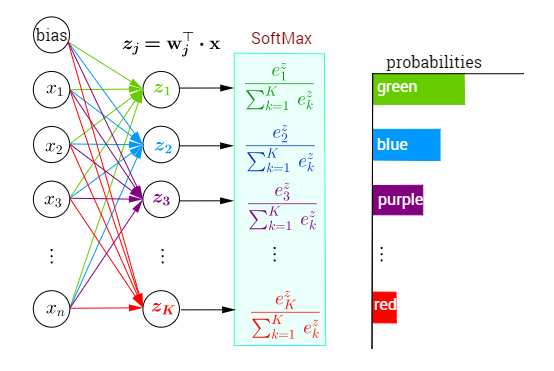
\includegraphics[width=10cm]{softmax.png}
  \caption{Multi-class classification with Neural Network and Softmax function}
\end{figure}

Softmax function for classification problem:

\begin{equation}
  \hat{y}_j = a_j^{(L)}=\dfrac{\exp(z_j^{(L)})}{\sum_{k=1}^{d^{(L)}}\exp(z_k^{(L)})}, j=1,\dots, d^{(L)}
\end{equation}

\begin{equation}
  \begin{aligned}
    \dfrac{\partial a_j^{(L)}}{\partial z_j^{(L)}}&=\dfrac{\exp(z_j^{(L)})\sum_{k=1}^{d^{(L)}}\exp(z_k^{(L)}) - \exp(z_j^{(L)})\exp(z_j^{(L)})}{\Bigg(\sum_{k=1}^{d^{(L)}}\exp(z_k^{(L)})\Bigg)^2}\\&=a_j^{(L)}\Big(1- a_j^{(L)} \Big)=\hat{y}_j \Big(1 - \hat{y}_j\Big)
  \end{aligned}
\end{equation}

Softmax cross entropy loss:

\begin{equation}
  \mathcal{L}=\sum_{j=1}^{d^{(L)}}-y_j \log a_j^{(L)}-(1-y_j)\log(1-a_j^{(L)})
\end{equation}

Compute partial derivatives of cross entropy loss with respect to $\bold{z}^{(L)}$:

\begin{equation}
  \begin{aligned}
    \dfrac{\partial \mathcal{L}}{\partial a_j^{(L)}}&=-\dfrac{y_j}{a_j^{(L)}}+\dfrac{1-y_j}{1-a_j^{(L)}}\\&=\dfrac{-y_j\Big(1-a_j^{(L)}\Big)+(1-y_j)a_j^{(L)}}{a_j^{(L)}\Big(1-a_j^{(L)}\Big)}\\&=\dfrac{a_j^{(L)}-y_j}{a_j^{(L)}\Big(1-a_j^{(L)}\Big)}
  \end{aligned}
\end{equation}

\begin{equation}
  \begin{aligned}
    e_j^{(L)}&=\dfrac{\partial \mathcal{L}}{\partial z_j^{(L)}}\\&=\dfrac{\partial \mathcal{L}}{\partial a_j^{(L)}}\dfrac{\partial a_j^{(L)}}{\partial z_j^{(L)}}\\&=\dfrac{a_j^{(L)}-y_j}{a_j^{(L)}\Big(1-a_j^{(L)}\Big)}a_j^{(L)}\Big(1- a_j^{(L)} \Big)\\&=a_j^{(L)} - y_j =\hat{y}_j - y_j
  \end{aligned}
\end{equation}

\begin{equation}
  \begin{aligned}
    \bold{e}^{(L)}&=\begin{bmatrix} a_1^{(L)} - y_1 & a_2^{(L)} - y_2 & \dots & a_j^{(L)} - y_j & \dots & a_{d^{(L)}}^{(L)} - y_{d^{(L)}} \end{bmatrix}^T\\&=\begin{bmatrix} \hat{y}_1 - y_1 & \hat{y}_2 - y_2 & \dots & \hat{y}_j - y_j & \dots & \hat{y}_{d^{(L)}} - y_{d^{(L)}} \end{bmatrix}^T
  \end{aligned}
\end{equation}

\section{Experiment}

\subsection{Fashion Mnist Dataset}

The experiment uses the dataset \href{https://github.com/zalandoresearch/fashion-mnist}{Fashion Mnist} which contains 70,000 grayscale images in 10 categories
The Fashion Mnist clothing dataset is a new standard one used in computer vision (CV) and deep learning (DL).

Although the dataset is relatively simple, it can be used as the basis for learning and practicing how to develop, evaluate, and use deep convolutional neural networks for image classification from scratch. 
This includes how to develop a robust test harness for estimating the performance of the model, how to explore improvements to the model, and how to save the model and later load it to make predictions on new data.
The images show individual articles of clothing at low resolution (28 x 28 pixels)

Divided into two sets:
\begin{itemize}
	  \item Training set contains 60000 images and correspoding labels
		\item Test set contains 10000 images and correspoding labels
\end{itemize}

The images are 28x28 NumPy arrays, with pixel values ranging from 0 to 255. 
	
The labels are an array of integers, ranging from 0 to 9. These correspond to the class of clothing the image represents:

\begin{table} [h!]
  \centering
  \begin{tabular}{ || c | c  || }
  \hline
  Label & Class \\ [0.5 ex]
  \hline \hline
  0 & T-shirt/top \\ \hline
  1 & Trouser \\ \hline
  2 & Pullover \\ \hline
  3 & Dress \\ \hline
  4 & Coat \\ \hline
  5 & Sandal\\ \hline
  6 & Shirt\\ \hline 
  7 & Sneaker \\ \hline
  8 & Bag \\ \hline
  9 & Ankle boot \\ [1ex]
  \hline
  \end{tabular}
  \caption{Mapping label to class name}
\end{table}

It is a more challenging classification problem than MNIST and top results are achieved by deep learning convolutional neural networks with a classification accuracy of about 90\% to 95\% on the hold out test dataset.

\begin{figure}[h!]
  \centering
  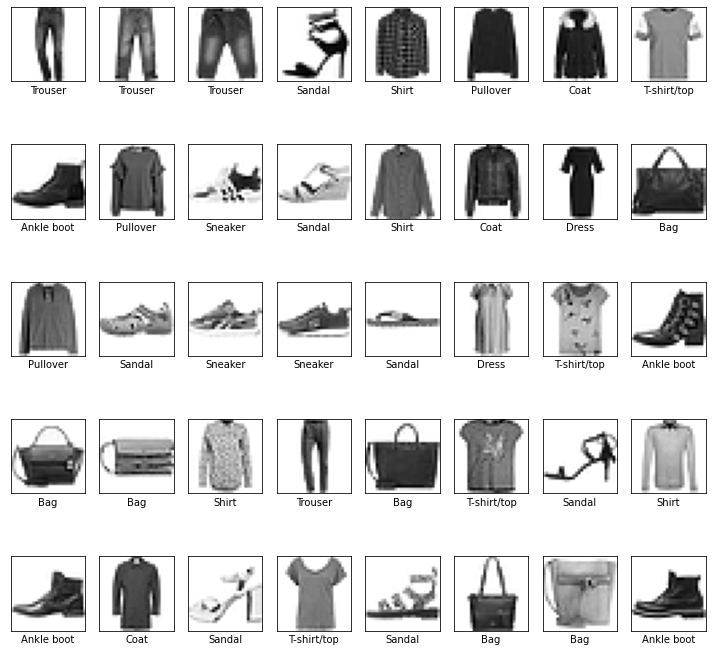
\includegraphics[width=8cm]{sample_images_with_labels.png}
  \caption{Sample images with labels}
\end{figure}

Fashion Mnist was proposed to be a replacement for MNIST, and although it has not been solved, it is possible to routinely achieve error rates of 10\% or less. 
Like MNIST, it can be a useful starting point for developing and practicing a methodology for solving image classification using neural networks.

Instead of reviewing the literature on well-performing models on the dataset, we can develop a new model from scratch.
The dataset already has a well-defined train and test dataset that we can use.

\subsection{Data Loading}

For example, we know that the images are all pre-segmented (e.g. each image contains a single item of clothing), that the images all have the same square size of 28x28 pixels, and that the images are grayscale. Therefore, we can load the images and reshape the data arrays to have a single color channel.

We also know that there are 10 classes and that classes are represented as unique integers.
We can, therefore, use a one hot encoding for the class element of each sample, transforming the integer into a 10 element binary vector with a 1 for the index of the class value.

The pixel values for each image in the dataset are unsigned integers in the range between black and white, or 0 and 255.
We do not know the best way to scale the pixel values for modeling, but we know that some scaling will be required.
A good starting point is to normalize the pixel values of grayscale images, e.g. rescale them to the range [0,1]. 
This involves first converting the data type from unsigned integers to floats, then dividing the pixel values by the maximum value.

\subsection{Model training and analysis}

We define a fully connected neural network model for the experiment.
Our neural network contains 2 hidden layers. The input layer size 784-d (equals size of flattened input image),
the first hiddlen layer with 128 units followed by second hidden layer with the same number of units.
Given that the problem is a multi-class classification, we know that we will require an output layer with 10 units in order to predict the probability distribution of an image belonging to each of the 10 classes. 
This will also require the use of a softmax activation function.

Network architecture and hyperparameters:
\begin{itemize}
	  \item Input image is flattend to 784-d vector
		\item 2 hidden layers, there are 128 neurons in each layer
  	\item Output layer contains 10 neuron (equals number of class)
   	\item Activation function: ReLU
    \item Learning rate: $\lbrack 10^{-5}, 10^{-4}, 10^{-3}, 10^{-2}, 5\times10^{-2}, 10^{-1} \rbrack$
    \item Batch-size: 256
    \item Num training epochs: 250
\end{itemize}

\begin{figure}[h!]
  \centering
  \resizebox{12cm}{!}{
    \begin{tikzpicture}[x=2.2cm,y=1.4cm]
      \message{^^JNeural network, shifted}
      \readlist\Nnod{4,5,5,3} % array of number of nodes per layer
      \readlist\Nstr{784, 128, 128, 10} % array of string number of nodes per layer
      \readlist\Cstr{\strut x,a^{(\prev)},a^{(\prev)},\hat{y}} % array of coefficient symbol per layer
      \def\yshift{0.5} % shift last node for dots
      
      \message{^^J  Layer}
      \foreachitem \N \in \Nnod{ % loop over layers
        \def\lay{\Ncnt} % alias of index of current layer
        \pgfmathsetmacro\prev{int(\Ncnt-1)} % number of previous layer
        \message{\lay,}
        \foreach \i [evaluate={\c=int(\i==\N); \y=\N/2-\i-\c*\yshift;
               \index=(\i<\N?int(\i):"\Nstr[\lay]");
               \x=\lay; \n=\nstyle;}] in {1,...,\N}{ % loop over nodes
        % NODES
        \node[node \n] (N\lay-\i) at (\x,\y) {$\Cstr[\lay]_{\index}$};
        
        % CONNECTIONS
        \ifnum\lay>1 % connect to previous layer
          \foreach \j in {1,...,\Nnod[\prev]}{ % loop over nodes in previous layer
          \draw[connect,white,line width=1.2] (N\prev-\j) -- (N\lay-\i);
          \draw[connect] (N\prev-\j) -- (N\lay-\i);
          %\draw[connect] (N\prev-\j.0) -- (N\lay-\i.180); % connect to left
          }
        \fi % else: nothing to connect first layer
        
        }
        \path (N\lay-\N) --++ (0,1+\yshift) node[midway,scale=1.5] {$\vdots$};
      }
      
      % LABELS
      \node[above=0.5cm,align=center,mygreen!60!black] at (N1-1.90) {784-d input};
      \node[above=0.5cm,align=center,myblue!60!black] at (N2-1.90) {128 neurons};
      \node[above=0.5cm,align=center,myblue!60!black] at (N3-1.90) {128 neurons};
      \node[above=0.5cm,align=center,myred!60!black] at (N\Nnodlen-1.90) {10 classes};
      
    \end{tikzpicture}
  }
  \caption{Neural network architecture used in experiment}
\end{figure}

ReLU is our activation function after each hidden layers. We use He-Kaiming weight initialization scheme.
We use stochastic gradient descent with multiple bands of learning rate to find optimal learning rate.
The categorical cross-entropy loss function will be optimized, suitable for multi-class classification, and we will monitor the classification accuracy metric, which is appropriate given we have the same number of examples in each of the 10 classes.



\begin{figure}[h!]
  \centering
  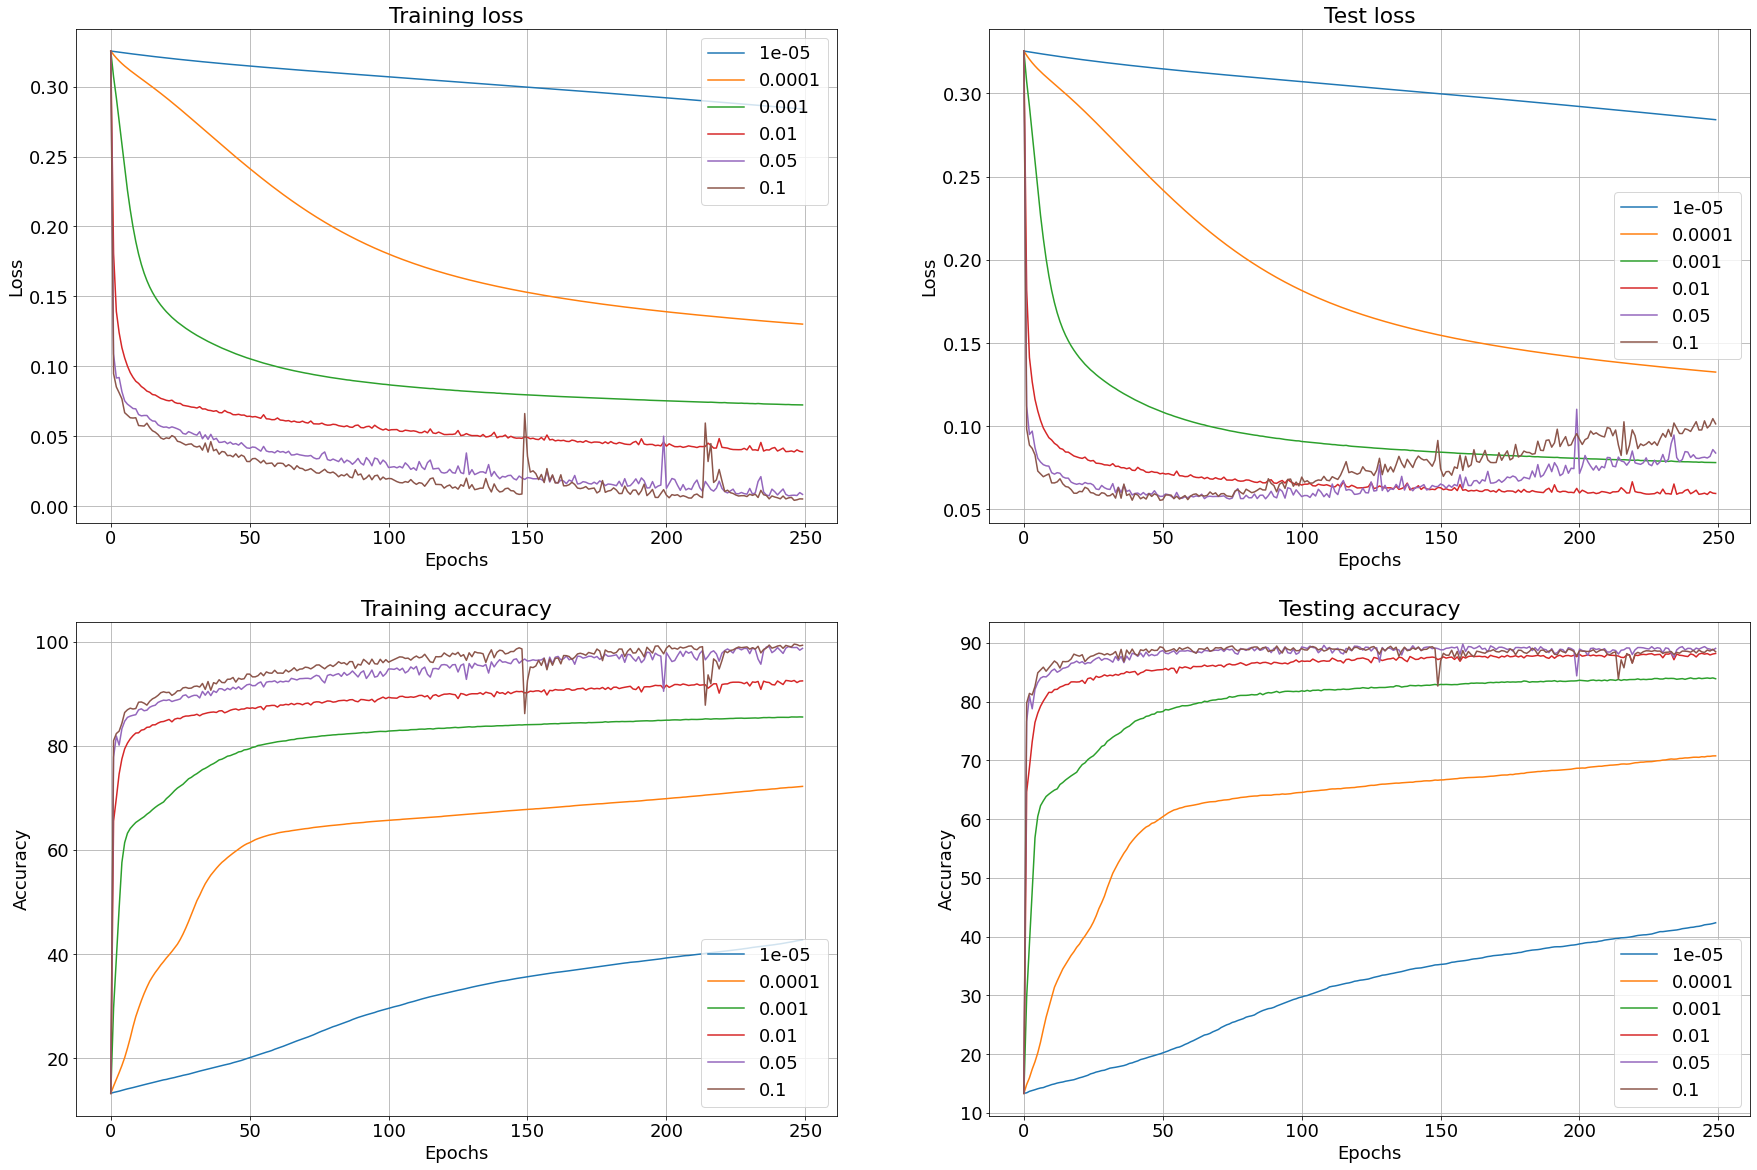
\includegraphics[width=15cm]{learning_rate_comparisons.png}
  \caption{Result with different learning rates}
  \label{fig:learning_rate}
\end{figure}

We train the model for 250 epochs for each learning rate. 
The results of the accuracy and the loss function are shown in figure \ref{fig:learning_rate}.

We find that with a low learning rate, the decrease in the loss function and the increase in accuracy are very slow. 
But with very large learning rate, the accuracy curve and loss function fluctuate greatly even leading to divergence.
We figure out a learning rate of about 0.01, the loss function on the test set decreases steadily and the accuracy on the test set increases the most. 
So we consider the learning rate 0.01 as the optimal learning rate

\begin{figure}[h!]
  \centering
  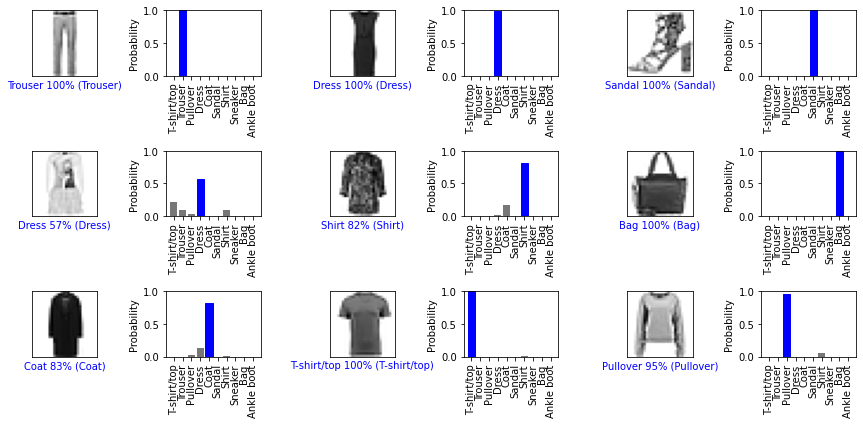
\includegraphics[width=12cm]{images_with_predictions_1.png}
  \caption{Images with prediction from trained neural network}
  \label{fig:predict_1}
\end{figure}

\begin{figure}[h!]
  \centering
  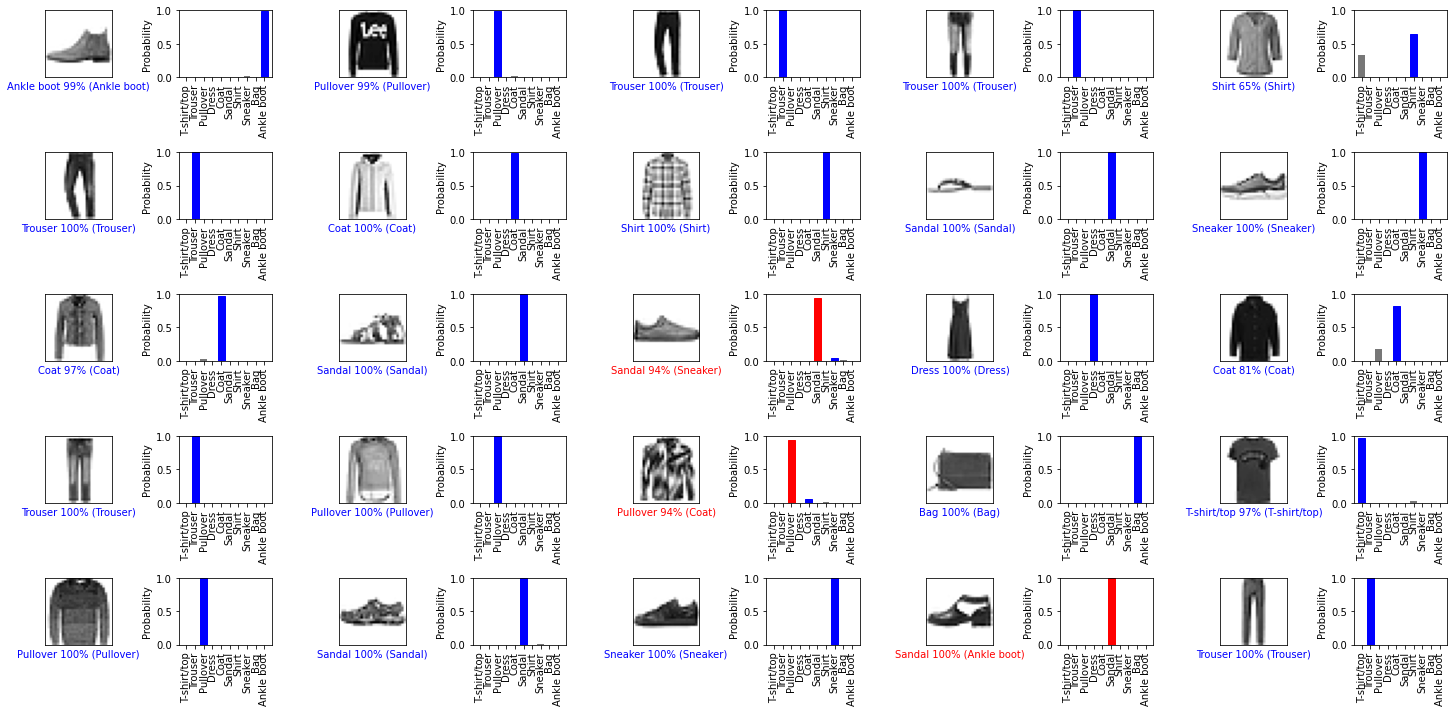
\includegraphics[width=15cm]{images_with_predictions_2.png}
  \caption{Images with prediction from trained neural network}
  \label{fig:predict_2}
\end{figure}

Figures \ref{fig:predict_1} and \ref{fig:predict_2} show the model's prediction results after being trained with the input images. 
The height of the column corresponding to a class is the probability that the model predicts that the input image belongs to the corresponding class. The blue column corresponds to the desired class. The red column corresponds to the class with the highest probability (as predicted by the model) not to coincide with the desired class. 
The gray columns are the classes with no highest probability and also not the desired class.


\begin{figure}[h!]
  \centering
  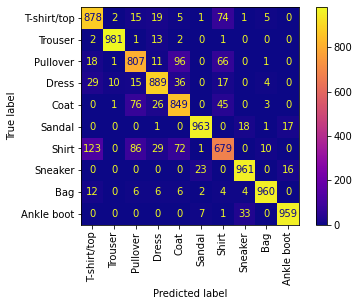
\includegraphics[width=12cm]{confusion_matrix.png}
  \caption{Confusion matrix}
  \label{fig:confusion_matrix}
\end{figure}

\begin{table} [h!]
  \centering
  \begin{tabular}{ || c | c | c | c | c|| }
  \hline
  Class & Precision & Recall & F1-score & Support \\ [0.5 ex]
  \hline \hline
  T-shirt/top & 0.827 & 0.878 & 0.851 & 1000 \\ \hline
  Trouser & 0.986 & 0.981 & 0.983 & 1000  \\ \hline
  Pullover & 0.802 & 0.807 & 0.805 & 1000 \\ \hline
  Dress & 0.894 & 0.889 & 0.892 & 1000 \\ \hline
  Coat & 0.796 & 0.849 & 0.822 & 1000 \\ \hline
  Sandal & 0.966 &0.963 & 0.964 & 1000\\ \hline
  Shirt & 0.766 & 0.679 & 0.720 & 1000\\ \hline 
  Sneaker & 0.945 & 0.961 & 0.953 & 1000 \\ \hline
  Bag &  0.976 & 0.960 & 0.968 & 1000 \\ \hline
  Ankle boot & 0.967 & 0.959 & 0.963 & 1000 \\ [1ex]
  \hline
  \end{tabular}
  \caption{Classification report of neural network on test set}
  \label{table:metrics}
\end{table}

Table \ref{table:metrics} shows the classification report of each class on the measures of accuracy, recall, F1-score, and the main support level is the number of elements corresponding to each class. 
We see that bag and sandal have the highest F-1 score because these classes look quite different from the rest.

Figure \ref{fig:confusion_matrix} shows the confusion matrix. 
The horizontal axis corresponds to the class predicted by the model, the vertical axis corresponds to the correct class. 
We observe that the Shirt class is often mistakenly predicted by the model as Tshirt/top and Pullover classes because these classes are quite similar.

\section{Conclusion and Future Direction}

In this essay, we have mentioned artificial neural networks and backpropagation algorithms. 
We have implemented the algorithm and applied it on the Fashion-Mnist dataset. 
However, this is only the simplest case in neural networks. In addition to the fully connected neural network structure, there are many other types of more complex and commonly used neural networks, especially convolutional neural networks. 
In the next steps of development, we will study convolutional neural networks and backpropagation algorithms for convolutional neural networks. 
The backpropagation algorithm for convolutional neural networks is not as simple as in the case of fully connected neural networks because a neuron is not connected to all neurons in the layer immediately preceding and succeeding it.
In addition, we need to study more about backpropagation algorithms in recurrent neural networks to model sequential data. 
The backpropagation algorithm in this type of neural network is extremely complicated, also known as backpropagation through time, which leads to difficult problems in neural network training such as gradient vanishing and gradient exploding.

\newpage
\addcontentsline{toc}{section}{References}
\printbibliography[title={References}]

\end{document}